\section{Results}
\label{sec:results}
In this section we present the results of the experiments defined in section \ref{sec:experiments}. The results will be grouped per scenario. We start by presenting overall damage of the system in each of the scenarios, as it is the key indicator of the performance of the system. We then present the other metrics that we defined in section \ref{ssec:metrics}.

\subsection{Scenario 1: No Changes}
\begin{figure}[H]
    \centering
    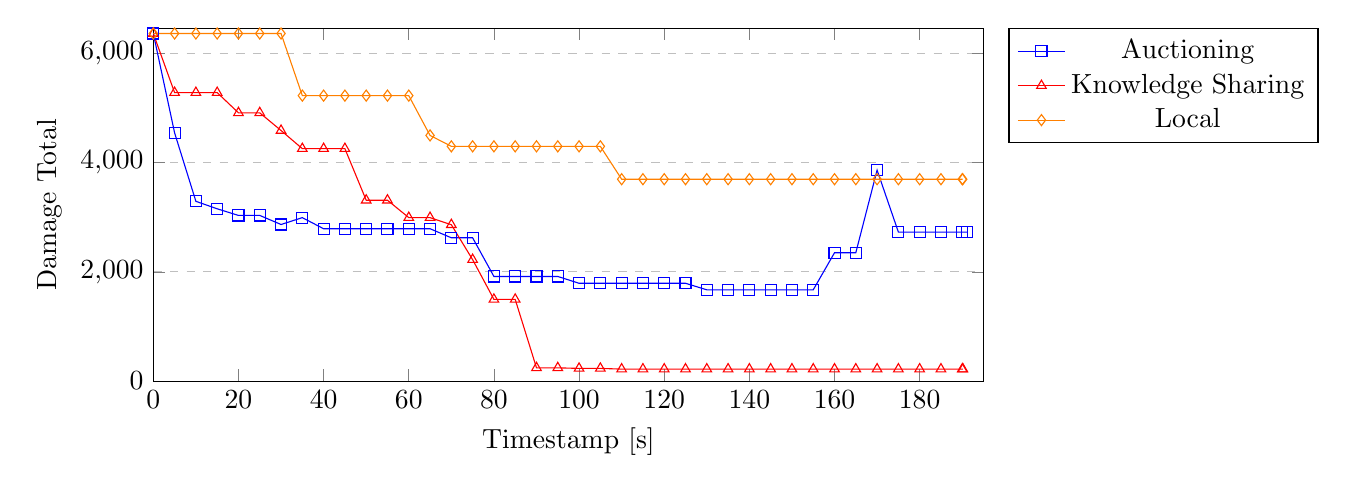
\begin{tikzpicture}
\begin{axis}[
    xlabel={Timestamp [s]},
    ylabel={Damage Total},
    xmin=0, xmax=195000,
    ymin=0, ymax=6464,
    legend pos=outer north east,
    ymajorgrids=true,
    grid style=dashed,
    width=\textwidth,
    height=0.5\textwidth,
    scaled x ticks=base 10:-3,
    xtick scale label code/.code={}
]

	\addplot[color=blue,mark=square] coordinates {
        (0,6367.26)(5000,4547.28)(10000,3293.02)(15000,3156.13)(20000,3034.57)(25000,3034.57)(30000,2868.58)(35000,2993.93)(40000,2790.80)(45000,2790.80)(50000,2790.80)(55000,2790.80)(60000,2790.80)(65000,2790.80)(70000,2624.98)(75000,2624.98)(80000,1916.52)(85000,1916.52)(90000,1916.52)(95000,1916.52)(100000,1791.72)(105000,1791.72)(110000,1791.72)(115000,1791.72)(120000,1791.72)(125000,1791.72)(130000,1671.71)(135000,1671.71)(140000,1671.71)(145000,1671.71)(150000,1671.71)(155000,1671.71)(160000,2351.16)(165000,2351.16)(170000,3864.46)(175000,2729.60)(180000,2729.60)(185000,2729.60)(190000,2729.60)(191066,2729.60)
    };
    \addlegendentry{Auctioning}
	\addplot[color=red,mark=triangle] coordinates {
        (0,6367.26)(5000,5284.52)(10000,5284.52)(15000,5284.52)(20000,4914.13)(25000,4914.13)(30000,4590.69)(35000,4257.62)(40000,4257.62)(45000,4257.62)(50000,3313.54)(55000,3313.54)(60000,2994.50)(65000,2994.50)(70000,2864.46)(75000,2224.62)(80000,1496.52)(85000,1496.52)(90000,242.72)(95000,242.72)(100000,232.18)(105000,232.18)(110000,219.25)(115000,219.25)(120000,219.25)(125000,219.25)(130000,219.25)(135000,219.25)(140000,219.25)(145000,219.25)(150000,219.25)(155000,219.25)(160000,219.25)(165000,219.25)(170000,219.25)(175000,219.25)(180000,219.25)(185000,219.25)(190000,219.25)(190155,219.25)
    };
    \addlegendentry{Knowledge Sharing}
	\addplot[color=orange,mark=diamond] coordinates {
        (0,6367.26)(5000,6367.26)(10000,6367.26)(15000,6367.26)(20000,6367.26)(25000,6367.26)(30000,6367.26)(35000,5229.23)(40000,5229.23)(45000,5229.23)(50000,5229.23)(55000,5229.23)(60000,5229.23)(65000,4499.97)(70000,4300.22)(75000,4300.22)(80000,4300.22)(85000,4300.22)(90000,4300.22)(95000,4300.22)(100000,4300.22)(105000,4300.22)(110000,3698.17)(115000,3698.17)(120000,3698.17)(125000,3698.17)(130000,3698.17)(135000,3698.17)(140000,3698.17)(145000,3698.17)(150000,3698.17)(155000,3698.17)(160000,3698.17)(165000,3698.17)(170000,3698.17)(175000,3698.17)(180000,3698.17)(185000,3698.17)(190000,3698.17)(190110,3698.17)
    };
    \addlegendentry{Local}




\end{axis}
\end{tikzpicture}
    \caption{This graph shows the overall damage of the system in the scenario where no changes are made overtime.}
    \label{fig:overall-damage-no-change}
\end{figure}
\begin{figure}[H]
    \centering
    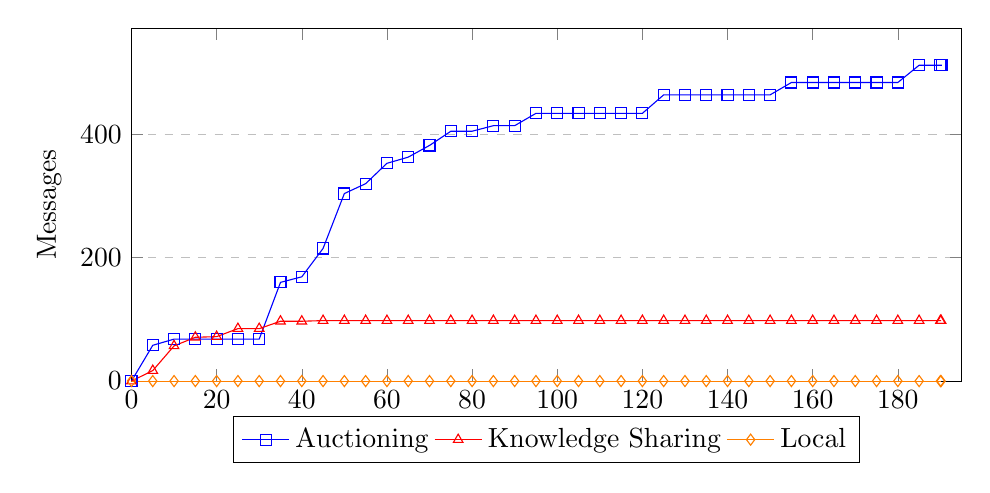
\begin{tikzpicture}
\begin{axis}[
    xlabel={Timestamp [s]},
    ylabel={Messages},
    xmin=0, xmax=195000,
    ymin=0, ymax=572,
    legend columns=-1,
    legend style={at={(0.5,-0.1)},anchor=north},
    ymajorgrids=true,
    grid style=dashed,
    width=\textwidth,
    height=0.5\textwidth,
    scaled x ticks=base 10:-3,
    xtick scale label code/.code={}
]

	\addplot[color=blue,mark=square] coordinates {
        (0,0)(5000,58)(10000,68)(15000,68)(20000,68)(25000,68)(30000,68)(35000,160)(40000,169)(45000,215)(50000,304)(55000,320)(60000,353)(65000,363)(70000,382)(75000,405)(80000,405)(85000,414)(90000,414)(95000,434)(100000,434)(105000,434)(110000,434)(115000,434)(120000,434)(125000,464)(130000,464)(135000,464)(140000,464)(145000,464)(150000,464)(155000,484)(160000,484)(165000,484)(170000,484)(175000,484)(180000,484)(185000,512)(190000,512)(190364,512)
    };
    \addlegendentry{Auctioning}
	\addplot[color=red,mark=triangle] coordinates {
        (0,0)(5000,17)(10000,57)(15000,71)(20000,72)(25000,85)(30000,85)(35000,97)(40000,97)(45000,98)(50000,98)(55000,98)(60000,98)(65000,98)(70000,98)(75000,98)(80000,98)(85000,98)(90000,98)(95000,98)(100000,98)(105000,98)(110000,98)(115000,98)(120000,98)(125000,98)(130000,98)(135000,98)(140000,98)(145000,98)(150000,98)(155000,98)(160000,98)(165000,98)(170000,98)(175000,98)(180000,98)(185000,98)(190000,98)(190165,98)
    };
    \addlegendentry{Knowledge Sharing}
	\addplot[color=orange,mark=diamond] coordinates {
        (0,0)(5000,0)(10000,0)(15000,0)(20000,0)(25000,0)(30000,0)(35000,0)(40000,0)(45000,0)(50000,0)(55000,0)(60000,0)(65000,0)(70000,0)(75000,0)(80000,0)(85000,0)(90000,0)(95000,0)(100000,0)(105000,0)(110000,0)(115000,0)(120000,0)(125000,0)(130000,0)(135000,0)(140000,0)(145000,0)(150000,0)(155000,0)(160000,0)(165000,0)(170000,0)(175000,0)(180000,0)(185000,0)(190000,0)(190150,0)
    };
    \addlegendentry{Local}




\end{axis}
\end{tikzpicture}
    \caption{Graph showing the total amount of messages sent between agents in the scenario where no changes are made overtime.}
\end{figure}
\begin{figure}[H]
    \centering
    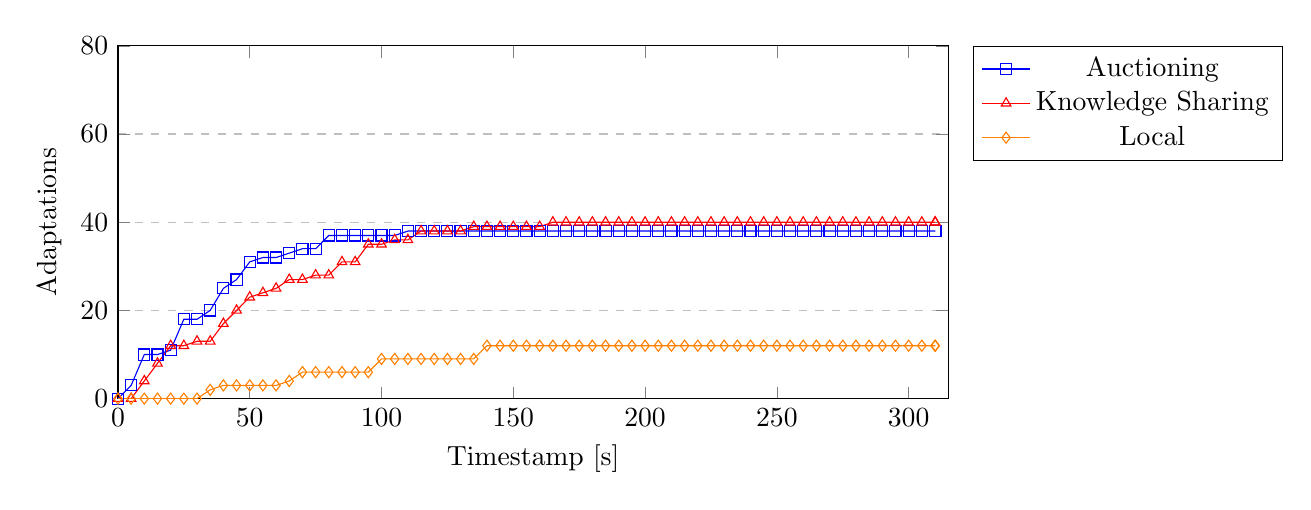
\begin{tikzpicture}
\begin{axis}[
    xlabel={Timestamp [s]},
    ylabel={Adaptations},
    xmin=0, xmax=315000,
    ymin=0, ymax=80,
    legend pos=outer north east,
    ymajorgrids=true,
    grid style=dashed,
    width=\textwidth,
    height=0.5\textwidth,
    scaled x ticks=base 10:-3,
    xtick scale label code/.code={}
]

	\addplot[color=blue,mark=square] coordinates {
        (0,0)(5000,3)(10000,10)(15000,10)(20000,11)(25000,18)(30000,18)(35000,20)(40000,25)(45000,27)(50000,31)(55000,32)(60000,32)(65000,33)(70000,34)(75000,34)(80000,37)(85000,37)(90000,37)(95000,37)(100000,37)(105000,37)(110000,38)(115000,38)(120000,38)(125000,38)(130000,38)(135000,38)(140000,38)(145000,38)(150000,38)(155000,38)(160000,38)(165000,38)(170000,38)(175000,38)(180000,38)(185000,38)(190000,38)(195000,38)(200000,38)(205000,38)(210000,38)(215000,38)(220000,38)(225000,38)(230000,38)(235000,38)(240000,38)(245000,38)(250000,38)(255000,38)(260000,38)(265000,38)(270000,38)(275000,38)(280000,38)(285000,38)(290000,38)(295000,38)(300000,38)(305000,38)(310000,38)(310169,38)
    };
    \addlegendentry{Auctioning}
	\addplot[color=red,mark=triangle] coordinates {
        (0,0)(5000,0)(10000,4)(15000,8)(20000,12)(25000,12)(30000,13)(35000,13)(40000,17)(45000,20)(50000,23)(55000,24)(60000,25)(65000,27)(70000,27)(75000,28)(80000,28)(85000,31)(90000,31)(95000,35)(100000,35)(105000,36)(110000,36)(115000,38)(120000,38)(125000,38)(130000,38)(135000,39)(140000,39)(145000,39)(150000,39)(155000,39)(160000,39)(165000,40)(170000,40)(175000,40)(180000,40)(185000,40)(190000,40)(195000,40)(200000,40)(205000,40)(210000,40)(215000,40)(220000,40)(225000,40)(230000,40)(235000,40)(240000,40)(245000,40)(250000,40)(255000,40)(260000,40)(265000,40)(270000,40)(275000,40)(280000,40)(285000,40)(290000,40)(295000,40)(300000,40)(305000,40)(310000,40)(310132,40)
    };
    \addlegendentry{Knowledge Sharing}
	\addplot[color=orange,mark=diamond] coordinates {
        (0,0)(5000,0)(10000,0)(15000,0)(20000,0)(25000,0)(30000,0)(35000,2)(40000,3)(45000,3)(50000,3)(55000,3)(60000,3)(65000,4)(70000,6)(75000,6)(80000,6)(85000,6)(90000,6)(95000,6)(100000,9)(105000,9)(110000,9)(115000,9)(120000,9)(125000,9)(130000,9)(135000,9)(140000,12)(145000,12)(150000,12)(155000,12)(160000,12)(165000,12)(170000,12)(175000,12)(180000,12)(185000,12)(190000,12)(195000,12)(200000,12)(205000,12)(210000,12)(215000,12)(220000,12)(225000,12)(230000,12)(235000,12)(240000,12)(245000,12)(250000,12)(255000,12)(260000,12)(265000,12)(270000,12)(275000,12)(280000,12)(285000,12)(290000,12)(295000,12)(300000,12)(305000,12)(310000,12)(310125,12)
    };
    \addlegendentry{Local}




\end{axis}
\end{tikzpicture}
    \caption{Graph showing the total amount of adaptations applied by agents in the scenario where no changes are made overtime.}
\end{figure}
\begin{figure}[H]
    \centering
        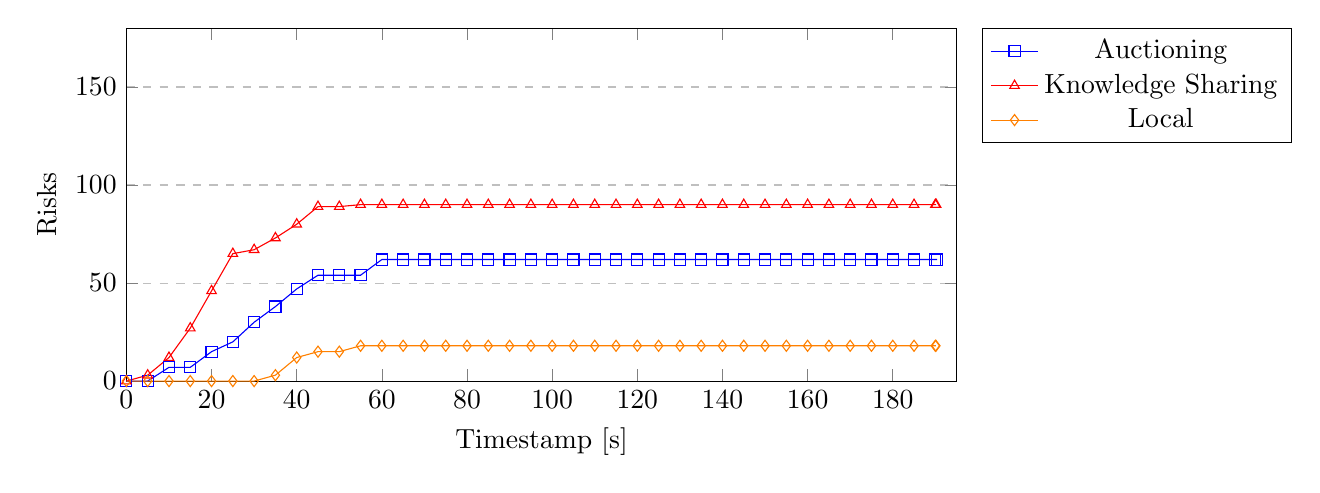
\begin{tikzpicture}
\begin{axis}[
    xlabel={Timestamp [s]},
    ylabel={Risks},
    xmin=0, xmax=195000,
    ymin=0, ymax=180,
    legend pos=outer north east,
    ymajorgrids=true,
    grid style=dashed,
    width=\textwidth,
    height=0.5\textwidth,
    scaled x ticks=base 10:-3,
    xtick scale label code/.code={}
]

	\addplot[color=blue,mark=square] coordinates {
        (0,0)(5000,0)(10000,7)(15000,7)(20000,15)(25000,20)(30000,30)(35000,38)(40000,47)(45000,54)(50000,54)(55000,54)(60000,62)(65000,62)(70000,62)(75000,62)(80000,62)(85000,62)(90000,62)(95000,62)(100000,62)(105000,62)(110000,62)(115000,62)(120000,62)(125000,62)(130000,62)(135000,62)(140000,62)(145000,62)(150000,62)(155000,62)(160000,62)(165000,62)(170000,62)(175000,62)(180000,62)(185000,62)(190000,62)(190434,62)
    };
    \addlegendentry{Auctioning}
	\addplot[color=red,mark=triangle] coordinates {
        (0,0)(5000,3)(10000,12)(15000,27)(20000,46)(25000,65)(30000,67)(35000,73)(40000,80)(45000,89)(50000,89)(55000,90)(60000,90)(65000,90)(70000,90)(75000,90)(80000,90)(85000,90)(90000,90)(95000,90)(100000,90)(105000,90)(110000,90)(115000,90)(120000,90)(125000,90)(130000,90)(135000,90)(140000,90)(145000,90)(150000,90)(155000,90)(160000,90)(165000,90)(170000,90)(175000,90)(180000,90)(185000,90)(190000,90)(190190,90)
    };
    \addlegendentry{Knowledge Sharing}
	\addplot[color=orange,mark=diamond] coordinates {
        (0,0)(5000,0)(10000,0)(15000,0)(20000,0)(25000,0)(30000,0)(35000,3)(40000,12)(45000,15)(50000,15)(55000,18)(60000,18)(65000,18)(70000,18)(75000,18)(80000,18)(85000,18)(90000,18)(95000,18)(100000,18)(105000,18)(110000,18)(115000,18)(120000,18)(125000,18)(130000,18)(135000,18)(140000,18)(145000,18)(150000,18)(155000,18)(160000,18)(165000,18)(170000,18)(175000,18)(180000,18)(185000,18)(190000,18)(190138,18)
    };
    \addlegendentry{Local}




\end{axis}
\end{tikzpicture}
    \caption{Graph showing the number of unique risks detected by agents in the scenario where no changes are made overtime.}
\end{figure}
\begin{figure}[H]
    \centering
        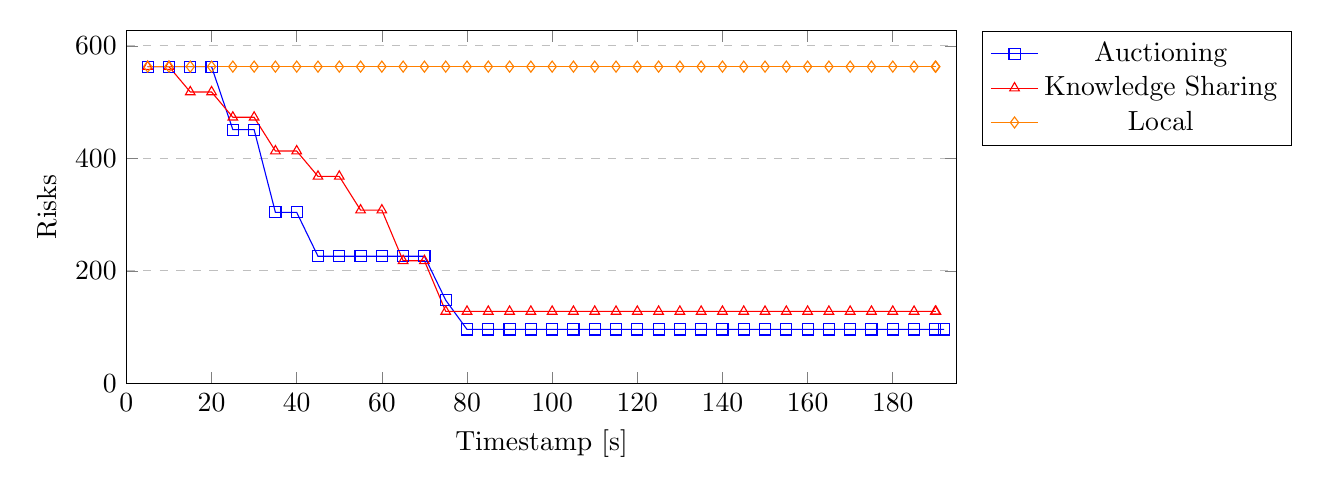
\begin{tikzpicture}
\begin{axis}[
    xlabel={Timestamp [s]},
    ylabel={Risks},
    xmin=0, xmax=195000,
    ymin=0, ymax=627,
    legend pos=outer north east,
    ymajorgrids=true,
    grid style=dashed,
    width=\textwidth,
    height=0.5\textwidth,
    scaled x ticks=base 10:-3,
    xtick scale label code/.code={}
]

	\addplot[color=blue,mark=square] coordinates {
        (5000,563)(10000,563)(15000,563)(20000,563)(25000,451)(30000,451)(35000,304)(40000,304)(45000,226)(50000,226)(55000,226)(60000,226)(65000,226)(70000,226)(75000,148)(80000,96)(85000,96)(90000,96)(95000,96)(100000,96)(105000,96)(110000,96)(115000,96)(120000,96)(125000,96)(130000,96)(135000,96)(140000,96)(145000,96)(150000,96)(155000,96)(160000,96)(165000,96)(170000,96)(175000,96)(180000,96)(185000,96)(190000,96)(192075,96)
    };
    \addlegendentry{Auctioning}
	\addplot[color=red,mark=triangle] coordinates {
        (5000,563)(10000,563)(15000,518)(20000,518)(25000,473)(30000,473)(35000,413)(40000,413)(45000,368)(50000,368)(55000,308)(60000,308)(65000,218)(70000,218)(75000,128)(80000,128)(85000,128)(90000,128)(95000,128)(100000,128)(105000,128)(110000,128)(115000,128)(120000,128)(125000,128)(130000,128)(135000,128)(140000,128)(145000,128)(150000,128)(155000,128)(160000,128)(165000,128)(170000,128)(175000,128)(180000,128)(185000,128)(190000,128)(190125,128)
    };
    \addlegendentry{Knowledge Sharing}
	\addplot[color=orange,mark=diamond] coordinates {
        (5000,563)(10000,563)(15000,563)(20000,563)(25000,563)(30000,563)(35000,563)(40000,563)(45000,563)(50000,563)(55000,563)(60000,563)(65000,563)(70000,563)(75000,563)(80000,563)(85000,563)(90000,563)(95000,563)(100000,563)(105000,563)(110000,563)(115000,563)(120000,563)(125000,563)(130000,563)(135000,563)(140000,563)(145000,563)(150000,563)(155000,563)(160000,563)(165000,563)(170000,563)(175000,563)(180000,563)(185000,563)(190000,563)(190111,563)
    };
    \addlegendentry{Local}




\end{axis}
\end{tikzpicture}
    \caption{Graph showing the number of remaining risks in the infrastructure in the scenario where no changes are made overtime.}
\end{figure}
\begin{figure}[H]
    \centering
        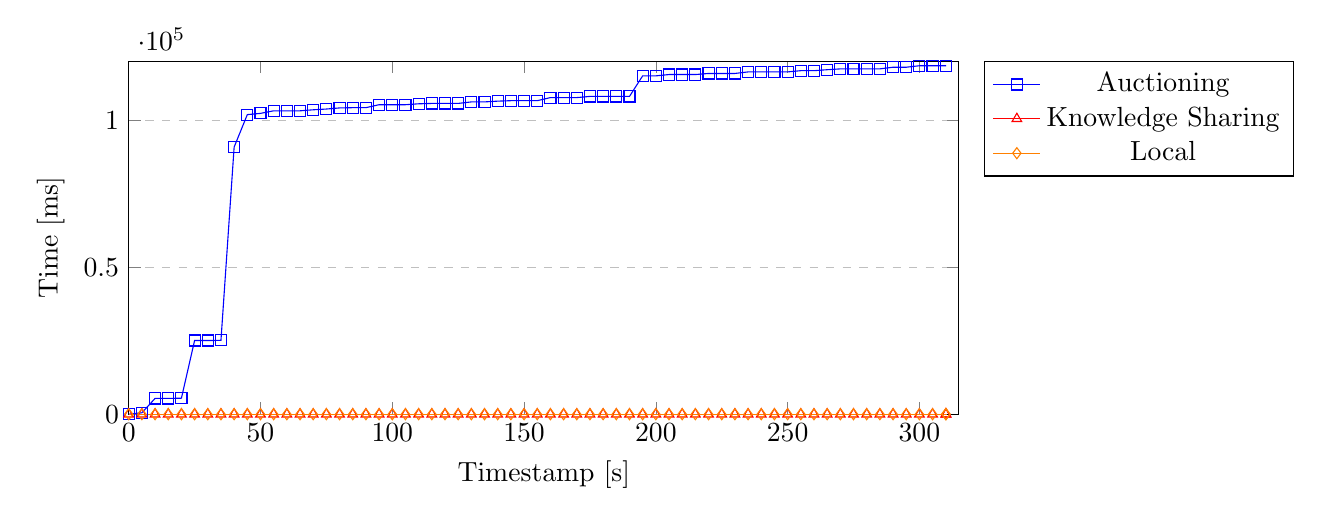
\begin{tikzpicture}
\begin{axis}[
    xlabel={Timestamp [s]},
    ylabel={Time [ms]},
    xmin=0, xmax=315000,
    ymin=0, ymax=120012,
    legend pos=outer north east,
    ymajorgrids=true,
    grid style=dashed,
    width=\textwidth,
    height=0.5\textwidth,
    scaled x ticks=base 10:-3,
    xtick scale label code/.code={}
]

	\addplot[color=blue,mark=square] coordinates {
        (0,0)(5000,475)(10000,5361)(15000,5361)(20000,5440)(25000,25066)(30000,25066)(35000,25093)(40000,90854)(45000,101889)(50000,102312)(55000,103185)(60000,103185)(65000,103185)(70000,103531)(75000,103788)(80000,104161)(85000,104251)(90000,104251)(95000,105263)(100000,105263)(105000,105263)(110000,105569)(115000,105695)(120000,105695)(125000,105695)(130000,106214)(135000,106214)(140000,106472)(145000,106629)(150000,106629)(155000,106629)(160000,107679)(165000,107679)(170000,107679)(175000,108080)(180000,108080)(185000,108080)(190000,108080)(195000,115072)(200000,115072)(205000,115518)(210000,115518)(215000,115518)(220000,115892)(225000,115892)(230000,115892)(235000,116415)(240000,116415)(245000,116415)(250000,116415)(255000,116836)(260000,116836)(265000,117162)(270000,117444)(275000,117444)(280000,117444)(285000,117444)(290000,118009)(295000,118009)(300000,118509)(305000,118509)(310000,118509)(310169,118509)
    };
    \addlegendentry{Auctioning}
	\addplot[color=red,mark=triangle] coordinates {
        (0,0)(5000,0)(10000,0)(15000,0)(20000,0)(25000,0)(30000,0)(35000,0)(40000,0)(45000,0)(50000,0)(55000,0)(60000,0)(65000,0)(70000,0)(75000,0)(80000,0)(85000,0)(90000,0)(95000,0)(100000,0)(105000,0)(110000,0)(115000,0)(120000,0)(125000,0)(130000,0)(135000,0)(140000,0)(145000,0)(150000,0)(155000,0)(160000,0)(165000,0)(170000,0)(175000,0)(180000,0)(185000,0)(190000,0)(195000,0)(200000,0)(205000,0)(210000,0)(215000,0)(220000,0)(225000,0)(230000,0)(235000,0)(240000,0)(245000,0)(250000,0)(255000,0)(260000,0)(265000,0)(270000,0)(275000,0)(280000,0)(285000,0)(290000,0)(295000,0)(300000,0)(305000,0)(310000,0)(310132,0)
    };
    \addlegendentry{Knowledge Sharing}
	\addplot[color=orange,mark=diamond] coordinates {
        (0,0)(5000,0)(10000,0)(15000,0)(20000,0)(25000,0)(30000,0)(35000,0)(40000,0)(45000,0)(50000,0)(55000,0)(60000,0)(65000,0)(70000,0)(75000,0)(80000,0)(85000,0)(90000,0)(95000,0)(100000,0)(105000,0)(110000,0)(115000,0)(120000,0)(125000,0)(130000,0)(135000,0)(140000,0)(145000,0)(150000,0)(155000,0)(160000,0)(165000,0)(170000,0)(175000,0)(180000,0)(185000,0)(190000,0)(195000,0)(200000,0)(205000,0)(210000,0)(215000,0)(220000,0)(225000,0)(230000,0)(235000,0)(240000,0)(245000,0)(250000,0)(255000,0)(260000,0)(265000,0)(270000,0)(275000,0)(280000,0)(285000,0)(290000,0)(295000,0)(300000,0)(305000,0)(310000,0)(310125,0)
    };
    \addlegendentry{Local}




\end{axis}
\end{tikzpicture}
    \caption{Graph showing the sum of time spent auctioning by agents in the scenario where no changes are made overtime.}
\end{figure}
\begin{figure}[H]
    \centering
        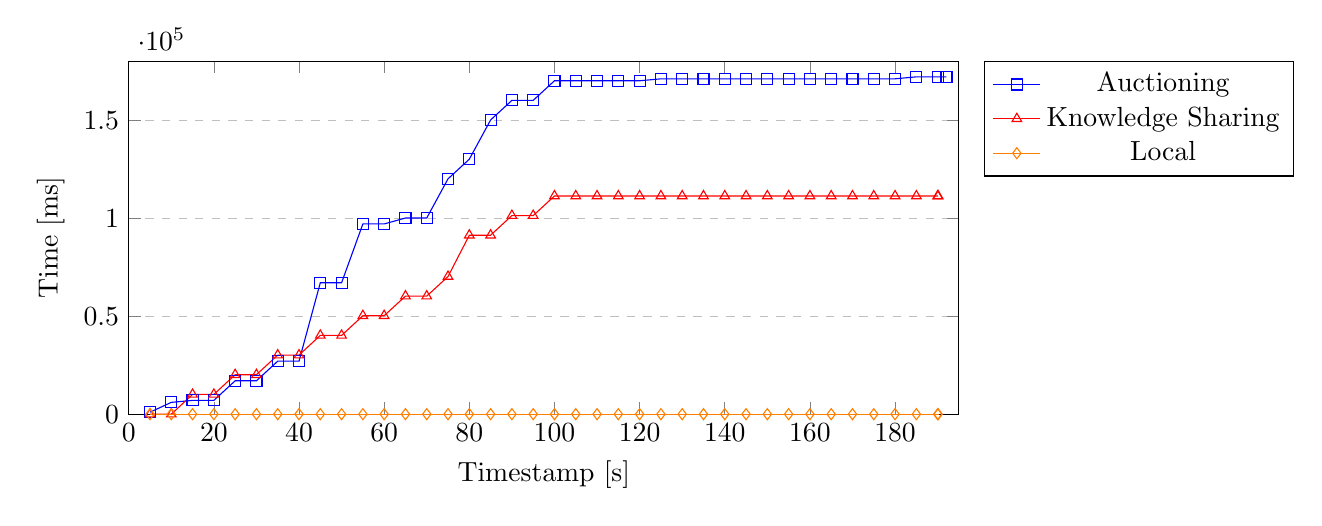
\begin{tikzpicture}
\begin{axis}[
    xlabel={Timestamp [s]},
    ylabel={Time [ms]},
    xmin=0, xmax=195000,
    ymin=0, ymax=180018,
    legend pos=outer north east,
    ymajorgrids=true,
    grid style=dashed,
    width=\textwidth,
    height=0.5\textwidth,
    scaled x ticks=base 10:-3,
    xtick scale label code/.code={}
]

	\addplot[color=blue,mark=square] coordinates {
        (5000,1004)(10000,6025)(15000,7027)(20000,7027)(25000,17033)(30000,17033)(35000,27038)(40000,27038)(45000,67055)(50000,67055)(55000,97062)(60000,97062)(65000,100075)(70000,100075)(75000,120080)(80000,130084)(85000,150091)(90000,160095)(95000,160095)(100000,170098)(105000,170098)(110000,170098)(115000,170098)(120000,170098)(125000,171100)(130000,171100)(135000,171100)(140000,171100)(145000,171100)(150000,171100)(155000,171100)(160000,171100)(165000,171100)(170000,171100)(175000,171100)(180000,171100)(185000,172103)(190000,172103)(192075,172103)
    };
    \addlegendentry{Auctioning}
	\addplot[color=red,mark=triangle] coordinates {
        (5000,0)(10000,0)(15000,10085)(20000,10085)(25000,20130)(30000,20130)(35000,30153)(40000,30153)(45000,40192)(50000,40192)(55000,50224)(60000,50224)(65000,60229)(70000,60229)(75000,70233)(80000,91314)(85000,91314)(90000,101317)(95000,101317)(100000,111324)(105000,111324)(110000,111324)(115000,111324)(120000,111324)(125000,111324)(130000,111324)(135000,111324)(140000,111324)(145000,111324)(150000,111324)(155000,111324)(160000,111324)(165000,111324)(170000,111324)(175000,111324)(180000,111324)(185000,111324)(190000,111324)(190125,111324)
    };
    \addlegendentry{Knowledge Sharing}
	\addplot[color=orange,mark=diamond] coordinates {
        (5000,0)(10000,0)(15000,0)(20000,0)(25000,0)(30000,0)(35000,0)(40000,0)(45000,0)(50000,0)(55000,0)(60000,0)(65000,0)(70000,0)(75000,0)(80000,0)(85000,0)(90000,0)(95000,0)(100000,0)(105000,0)(110000,0)(115000,0)(120000,0)(125000,0)(130000,0)(135000,0)(140000,0)(145000,0)(150000,0)(155000,0)(160000,0)(165000,0)(170000,0)(175000,0)(180000,0)(185000,0)(190000,0)(190111,0)
    };
    \addlegendentry{Local}




\end{axis}
\end{tikzpicture}
    \caption{Graph showing the sum of time spent adapting by agents in the scenario where no changes are made overtime.}
\end{figure}


\subsection{Scenario 2: Risk Introduction}
\begin{figure}[H]
    \centering
    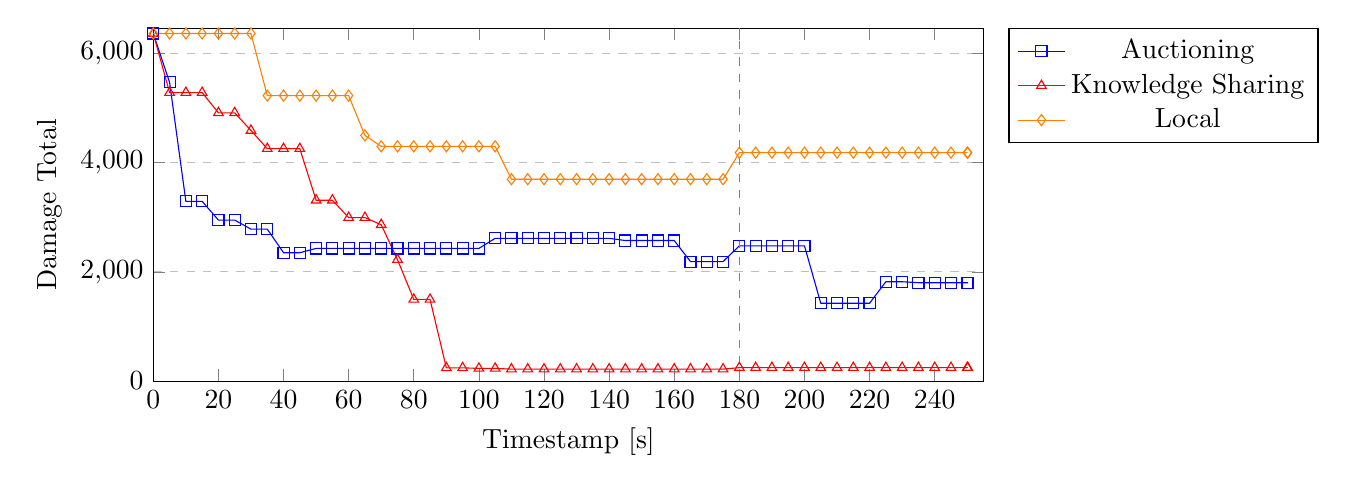
\begin{tikzpicture}
\begin{axis}[
    xlabel={Timestamp [s]},
    ylabel={Damage Total},
    xmin=0, xmax=255000,
    ymin=0, ymax=6464,
    legend pos=outer north east,
    ymajorgrids=true,
    grid style=dashed,
    width=\textwidth,
    height=0.5\textwidth,
    scaled x ticks=base 10:-3,
    xtick scale label code/.code={}
]

	\addplot[color=blue,mark=square] coordinates {
        (0,6367.26)(5000,5473.92)(10000,3293.02)(15000,3293.02)(20000,2949.34)(25000,2949.34)(30000,2783.36)(35000,2783.36)(40000,2351.49)(45000,2351.49)(50000,2430.01)(55000,2430.01)(60000,2430.01)(65000,2430.01)(70000,2430.01)(75000,2430.01)(80000,2430.01)(85000,2430.01)(90000,2430.01)(95000,2430.01)(100000,2430.01)(105000,2615.26)(110000,2615.26)(115000,2615.26)(120000,2615.26)(125000,2615.26)(130000,2615.26)(135000,2615.26)(140000,2615.26)(145000,2574.45)(150000,2574.45)(155000,2574.45)(160000,2574.45)(165000,2188.56)(170000,2188.56)(175000,2188.56)(180000,2477.58)(185000,2477.58)(190000,2477.58)(195000,2477.58)(200000,2477.58)(205000,1426.19)(210000,1426.19)(215000,1426.19)(220000,1426.19)(225000,1819.63)(230000,1819.63)(235000,1802.13)(240000,1802.13)(245000,1802.13)(250000,1802.13)(250288,1802.13)
    };
    \addlegendentry{Auctioning}
	\addplot[color=red,mark=triangle] coordinates {
        (0,6367.26)(5000,5284.52)(10000,5284.52)(15000,5284.52)(20000,4914.13)(25000,4914.13)(30000,4590.69)(35000,4257.62)(40000,4257.62)(45000,4257.62)(50000,3313.54)(55000,3313.54)(60000,2994.50)(65000,2994.50)(70000,2864.46)(75000,2224.62)(80000,1496.52)(85000,1496.52)(90000,242.72)(95000,242.72)(100000,232.18)(105000,232.18)(110000,219.25)(115000,219.25)(120000,219.25)(125000,219.25)(130000,219.25)(135000,219.25)(140000,219.25)(145000,219.25)(150000,219.25)(155000,219.25)(160000,219.25)(165000,219.25)(170000,219.25)(175000,219.25)(180000,245.68)(185000,245.68)(190000,245.68)(195000,245.68)(200000,245.68)(205000,245.68)(210000,245.68)(215000,245.68)(220000,245.68)(225000,245.68)(230000,245.68)(235000,245.68)(240000,245.68)(245000,245.68)(250000,245.68)(250159,245.68)
    };
    \addlegendentry{Knowledge Sharing}
	\addplot[color=orange,mark=diamond] coordinates {
        (0,6367.26)(5000,6367.26)(10000,6367.26)(15000,6367.26)(20000,6367.26)(25000,6367.26)(30000,6367.26)(35000,5229.23)(40000,5229.23)(45000,5229.23)(50000,5229.23)(55000,5229.23)(60000,5229.23)(65000,4499.97)(70000,4300.22)(75000,4300.22)(80000,4300.22)(85000,4300.22)(90000,4300.22)(95000,4300.22)(100000,4300.22)(105000,4300.22)(110000,3698.17)(115000,3698.17)(120000,3698.17)(125000,3698.17)(130000,3698.17)(135000,3698.17)(140000,3698.17)(145000,3698.17)(150000,3698.17)(155000,3698.17)(160000,3698.17)(165000,3698.17)(170000,3698.17)(175000,3698.17)(180000,4184.36)(185000,4184.36)(190000,4184.36)(195000,4184.36)(200000,4184.36)(205000,4184.36)(210000,4184.36)(215000,4184.36)(220000,4184.36)(225000,4184.36)(230000,4184.36)(235000,4184.36)(240000,4184.36)(245000,4184.36)(250000,4184.36)(250135,4184.36)
    };
    \addlegendentry{Local}

	\addplot[color=gray, dashed,] coordinates {(180000,0) (180000,6464)};


\end{axis}
\end{tikzpicture}
    \caption{This graph shows the overall damage of the system in the risk introduction scenario. The damage is shown for each of the three strategies. The vertical lines indicate the time at which a risk is introduced.}
    \label{fig:overall-damage-inroduce-risk}
\end{figure}

\begin{figure}[H]
    \centering
    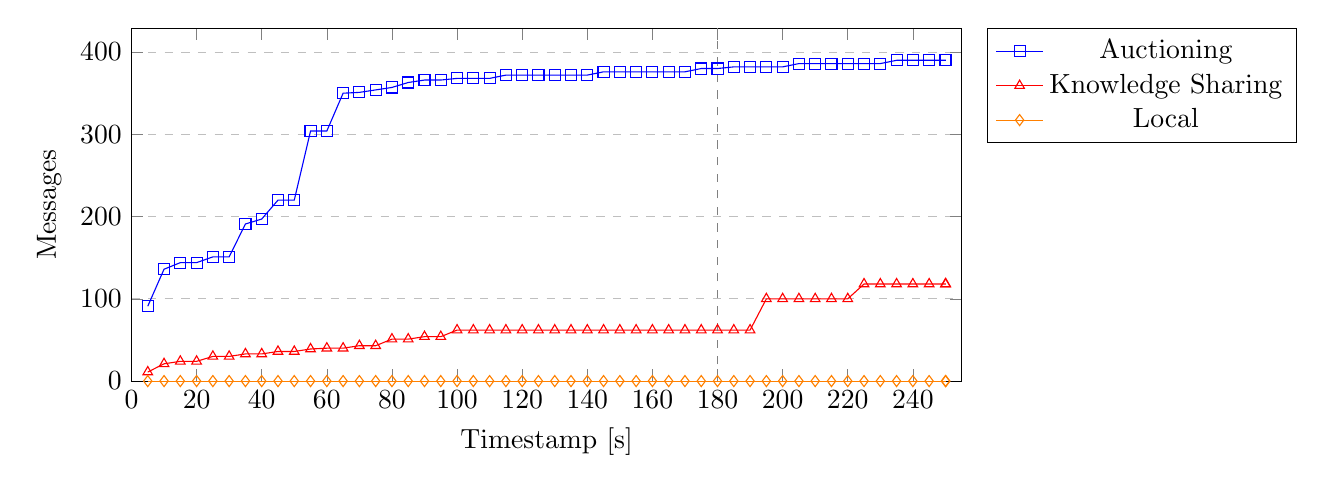
\begin{tikzpicture}
\begin{axis}[
    xlabel={Timestamp [s]},
    ylabel={Messages},
    xmin=0, xmax=255000,
    ymin=0, ymax=429,
    legend pos=outer north east,
    ymajorgrids=true,
    grid style=dashed,
    width=\textwidth,
    height=0.5\textwidth,
    scaled x ticks=base 10:-3,
    xtick scale label code/.code={}
]

	\addplot[color=blue,mark=square] coordinates {
        (5000,91)(10000,136)(15000,144)(20000,144)(25000,151)(30000,151)(35000,191)(40000,197)(45000,220)(50000,220)(55000,304)(60000,304)(65000,350)(70000,351)(75000,354)(80000,357)(85000,363)(90000,366)(95000,366)(100000,368)(105000,368)(110000,368)(115000,372)(120000,372)(125000,372)(130000,372)(135000,372)(140000,372)(145000,376)(150000,376)(155000,376)(160000,376)(165000,376)(170000,376)(175000,380)(180000,380)(185000,382)(190000,382)(195000,382)(200000,382)(205000,386)(210000,386)(215000,386)(220000,386)(225000,386)(230000,386)(235000,390)(240000,390)(245000,390)(250000,390)(250139,390)
    };
    \addlegendentry{Auctioning}
	\addplot[color=red,mark=triangle] coordinates {
        (5000,11)(10000,21)(15000,24)(20000,24)(25000,30)(30000,30)(35000,33)(40000,33)(45000,36)(50000,36)(55000,39)(60000,40)(65000,40)(70000,43)(75000,43)(80000,51)(85000,51)(90000,54)(95000,54)(100000,62)(105000,62)(110000,62)(115000,62)(120000,62)(125000,62)(130000,62)(135000,62)(140000,62)(145000,62)(150000,62)(155000,62)(160000,62)(165000,62)(170000,62)(175000,62)(180000,62)(185000,62)(190000,62)(195000,100)(200000,100)(205000,100)(210000,100)(215000,100)(220000,100)(225000,118)(230000,118)(235000,118)(240000,118)(245000,118)(250000,118)(250111,118)
    };
    \addlegendentry{Knowledge Sharing}
	\addplot[color=orange,mark=diamond] coordinates {
        (5000,0)(10000,0)(15000,0)(20000,0)(25000,0)(30000,0)(35000,0)(40000,0)(45000,0)(50000,0)(55000,0)(60000,0)(65000,0)(70000,0)(75000,0)(80000,0)(85000,0)(90000,0)(95000,0)(100000,0)(105000,0)(110000,0)(115000,0)(120000,0)(125000,0)(130000,0)(135000,0)(140000,0)(145000,0)(150000,0)(155000,0)(160000,0)(165000,0)(170000,0)(175000,0)(180000,0)(185000,0)(190000,0)(195000,0)(200000,0)(205000,0)(210000,0)(215000,0)(220000,0)(225000,0)(230000,0)(235000,0)(240000,0)(245000,0)(250000,0)(250115,0)
    };
    \addlegendentry{Local}

	\addplot[color=gray, dashed,] coordinates {(180000,0) (180000,429)};


\end{axis}
\end{tikzpicture}
    \caption{Graph showing the total amount of messages sent between agents in the risk introduction scenario.}
\end{figure}
\begin{figure}[H]
    \centering
    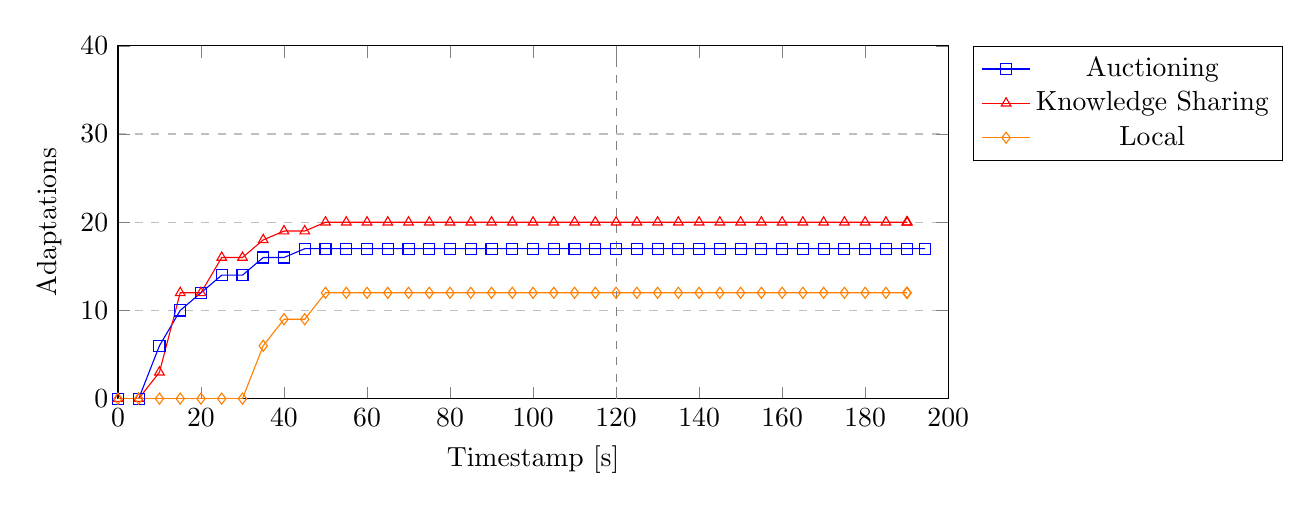
\begin{tikzpicture}
\begin{axis}[
    xlabel={Timestamp [s]},
    ylabel={Adaptations},
    xmin=0, xmax=200000,
    ymin=0, ymax=40,
    legend pos=outer north east,
    ymajorgrids=true,
    grid style=dashed,
    width=\textwidth,
    height=0.5\textwidth,
    scaled x ticks=base 10:-3,
    xtick scale label code/.code={}
]

	\addplot[color=blue,mark=square] coordinates {
        (0,0)(5000,0)(10000,6)(15000,10)(20000,12)(25000,14)(30000,14)(35000,16)(40000,16)(45000,17)(50000,17)(55000,17)(60000,17)(65000,17)(70000,17)(75000,17)(80000,17)(85000,17)(90000,17)(95000,17)(100000,17)(105000,17)(110000,17)(115000,17)(120000,17)(125000,17)(130000,17)(135000,17)(140000,17)(145000,17)(150000,17)(155000,17)(160000,17)(165000,17)(170000,17)(175000,17)(180000,17)(185000,17)(190000,17)(194444,17)
    };
    \addlegendentry{Auctioning}
	\addplot[color=red,mark=triangle] coordinates {
        (0,0)(5000,0)(10000,3)(15000,12)(20000,12)(25000,16)(30000,16)(35000,18)(40000,19)(45000,19)(50000,20)(55000,20)(60000,20)(65000,20)(70000,20)(75000,20)(80000,20)(85000,20)(90000,20)(95000,20)(100000,20)(105000,20)(110000,20)(115000,20)(120000,20)(125000,20)(130000,20)(135000,20)(140000,20)(145000,20)(150000,20)(155000,20)(160000,20)(165000,20)(170000,20)(175000,20)(180000,20)(185000,20)(190000,20)(190175,20)
    };
    \addlegendentry{Knowledge Sharing}
	\addplot[color=orange,mark=diamond] coordinates {
        (0,0)(5000,0)(10000,0)(15000,0)(20000,0)(25000,0)(30000,0)(35000,6)(40000,9)(45000,9)(50000,12)(55000,12)(60000,12)(65000,12)(70000,12)(75000,12)(80000,12)(85000,12)(90000,12)(95000,12)(100000,12)(105000,12)(110000,12)(115000,12)(120000,12)(125000,12)(130000,12)(135000,12)(140000,12)(145000,12)(150000,12)(155000,12)(160000,12)(165000,12)(170000,12)(175000,12)(180000,12)(185000,12)(190000,12)(190124,12)
    };
    \addlegendentry{Local}

	\addplot[color=gray, dashed,] coordinates {(120000,0) (120000,40)};


\end{axis}
\end{tikzpicture}
    \caption{Graph showing the total amount of adaptations applied by agents in the risk introduction scenario.}
\end{figure}
\begin{figure}[H]
    \centering
        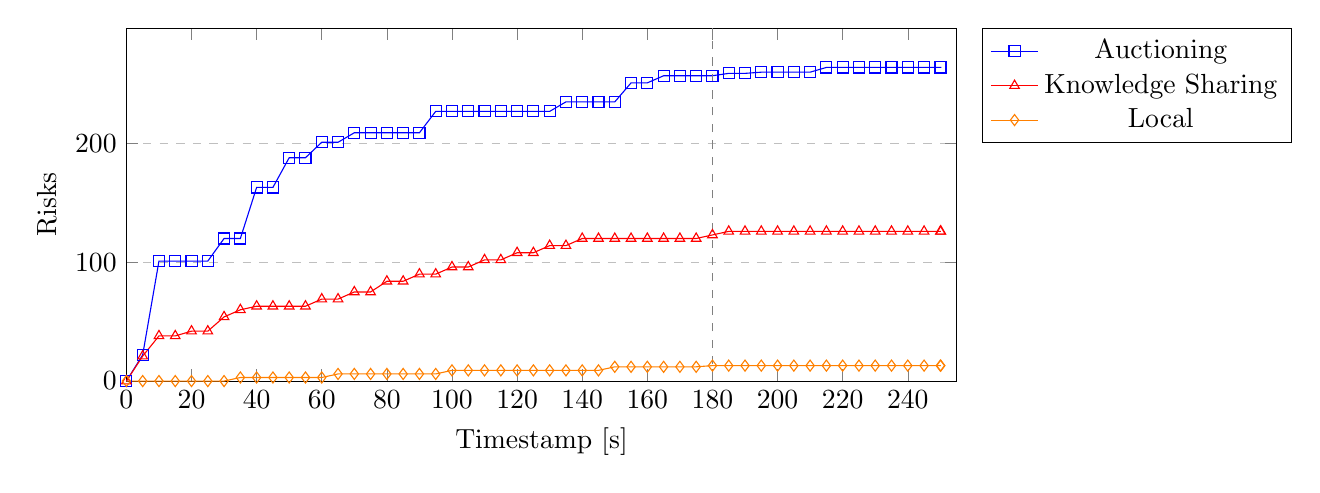
\begin{tikzpicture}
\begin{axis}[
    xlabel={Timestamp [s]},
    ylabel={Risks},
    xmin=0, xmax=255000,
    ymin=0, ymax=297,
    legend pos=outer north east,
    ymajorgrids=true,
    grid style=dashed,
    width=\textwidth,
    height=0.5\textwidth,
    scaled x ticks=base 10:-3,
    xtick scale label code/.code={}
]

	\addplot[color=blue,mark=square] coordinates {
        (0,0)(5000,22)(10000,101)(15000,101)(20000,101)(25000,101)(30000,120)(35000,120)(40000,163)(45000,163)(50000,188)(55000,188)(60000,201)(65000,201)(70000,209)(75000,209)(80000,209)(85000,209)(90000,209)(95000,227)(100000,227)(105000,227)(110000,227)(115000,227)(120000,227)(125000,227)(130000,227)(135000,235)(140000,235)(145000,235)(150000,235)(155000,251)(160000,251)(165000,257)(170000,257)(175000,257)(180000,257)(185000,259)(190000,259)(195000,260)(200000,260)(205000,260)(210000,260)(215000,264)(220000,264)(225000,264)(230000,264)(235000,264)(240000,264)(245000,264)(250000,264)(250288,264)
    };
    \addlegendentry{Auctioning}
	\addplot[color=red,mark=triangle] coordinates {
        (0,0)(5000,21)(10000,38)(15000,38)(20000,42)(25000,42)(30000,54)(35000,60)(40000,63)(45000,63)(50000,63)(55000,63)(60000,69)(65000,69)(70000,75)(75000,75)(80000,84)(85000,84)(90000,90)(95000,90)(100000,96)(105000,96)(110000,102)(115000,102)(120000,108)(125000,108)(130000,114)(135000,114)(140000,120)(145000,120)(150000,120)(155000,120)(160000,120)(165000,120)(170000,120)(175000,120)(180000,123)(185000,126)(190000,126)(195000,126)(200000,126)(205000,126)(210000,126)(215000,126)(220000,126)(225000,126)(230000,126)(235000,126)(240000,126)(245000,126)(250000,126)(250159,126)
    };
    \addlegendentry{Knowledge Sharing}
	\addplot[color=orange,mark=diamond] coordinates {
        (0,0)(5000,0)(10000,0)(15000,0)(20000,0)(25000,0)(30000,0)(35000,3)(40000,3)(45000,3)(50000,3)(55000,3)(60000,3)(65000,6)(70000,6)(75000,6)(80000,6)(85000,6)(90000,6)(95000,6)(100000,9)(105000,9)(110000,9)(115000,9)(120000,9)(125000,9)(130000,9)(135000,9)(140000,9)(145000,9)(150000,12)(155000,12)(160000,12)(165000,12)(170000,12)(175000,12)(180000,13)(185000,13)(190000,13)(195000,13)(200000,13)(205000,13)(210000,13)(215000,13)(220000,13)(225000,13)(230000,13)(235000,13)(240000,13)(245000,13)(250000,13)(250135,13)
    };
    \addlegendentry{Local}

	\addplot[color=gray, dashed,] coordinates {(180000,0) (180000,297)};


\end{axis}
\end{tikzpicture}
    \caption{Graph showing the number of unique risks detected by agents in the risk introduction scenario.}
\end{figure}
\begin{figure}[H]
    \centering
        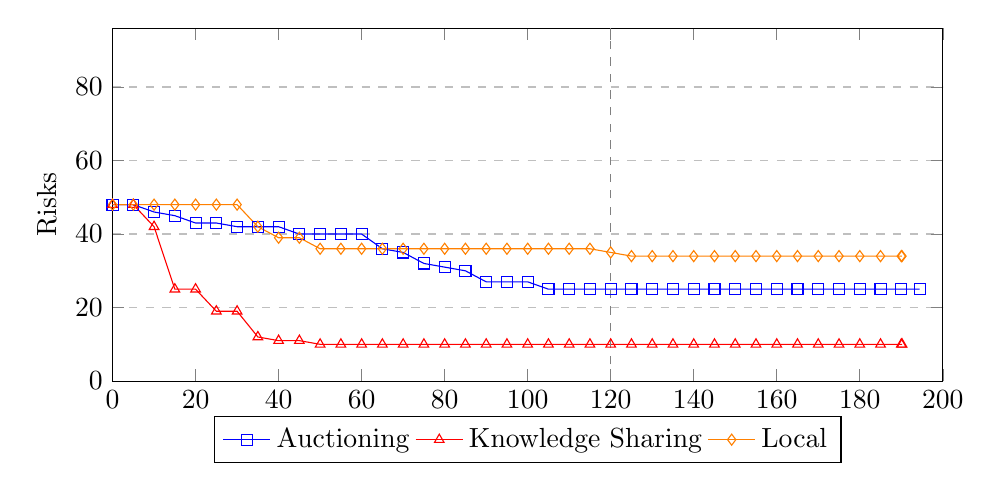
\begin{tikzpicture}
\begin{axis}[
    xlabel={Timestamp [s]},
    ylabel={Risks},
    xmin=0, xmax=200000,
    ymin=0, ymax=96,
    legend columns=-1,
    legend style={at={(0.5,-0.1)},anchor=north},
    ymajorgrids=true,
    grid style=dashed,
    width=\textwidth,
    height=0.5\textwidth,
    scaled x ticks=base 10:-3,
    xtick scale label code/.code={}
]

	\addplot[color=blue,mark=square] coordinates {
        (0,48)(5000,48)(10000,46)(15000,45)(20000,43)(25000,43)(30000,42)(35000,42)(40000,42)(45000,40)(50000,40)(55000,40)(60000,40)(65000,36)(70000,35)(75000,32)(80000,31)(85000,30)(90000,27)(95000,27)(100000,27)(105000,25)(110000,25)(115000,25)(120000,25)(125000,25)(130000,25)(135000,25)(140000,25)(145000,25)(150000,25)(155000,25)(160000,25)(165000,25)(170000,25)(175000,25)(180000,25)(185000,25)(190000,25)(194440,25)
    };
    \addlegendentry{Auctioning}
	\addplot[color=red,mark=triangle] coordinates {
        (0,48)(5000,48)(10000,42)(15000,25)(20000,25)(25000,19)(30000,19)(35000,12)(40000,11)(45000,11)(50000,10)(55000,10)(60000,10)(65000,10)(70000,10)(75000,10)(80000,10)(85000,10)(90000,10)(95000,10)(100000,10)(105000,10)(110000,10)(115000,10)(120000,10)(125000,10)(130000,10)(135000,10)(140000,10)(145000,10)(150000,10)(155000,10)(160000,10)(165000,10)(170000,10)(175000,10)(180000,10)(185000,10)(190000,10)(190192,10)
    };
    \addlegendentry{Knowledge Sharing}
	\addplot[color=orange,mark=diamond] coordinates {
        (0,48)(5000,48)(10000,48)(15000,48)(20000,48)(25000,48)(30000,48)(35000,42)(40000,39)(45000,39)(50000,36)(55000,36)(60000,36)(65000,36)(70000,36)(75000,36)(80000,36)(85000,36)(90000,36)(95000,36)(100000,36)(105000,36)(110000,36)(115000,36)(120000,35)(125000,34)(130000,34)(135000,34)(140000,34)(145000,34)(150000,34)(155000,34)(160000,34)(165000,34)(170000,34)(175000,34)(180000,34)(185000,34)(190000,34)(190162,34)
    };
    \addlegendentry{Local}

	\addplot[color=gray, dashed,] coordinates {(120000,0) (120000,96)};


\end{axis}
\end{tikzpicture}
    \caption{Graph showing the number of remaining risks in the infrastructure in the risk introduction scenario.}
\end{figure}
\begin{figure}[H]
    \centering
        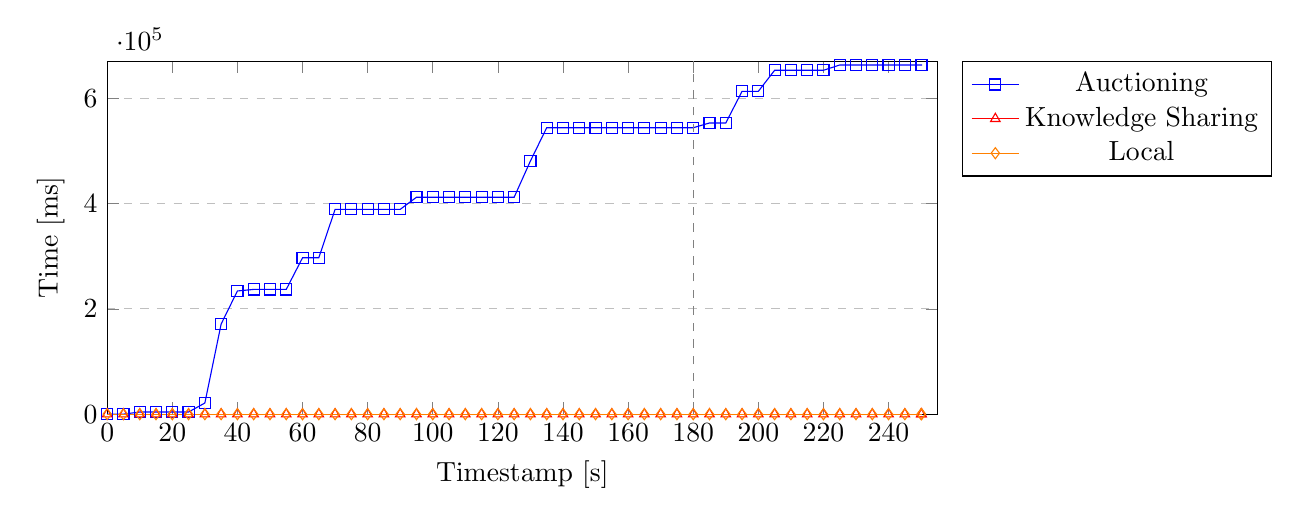
\begin{tikzpicture}
\begin{axis}[
    xlabel={Timestamp [s]},
    ylabel={Time [ms]},
    xmin=0, xmax=255000,
    ymin=0, ymax=670067,
    legend pos=outer north east,
    ymajorgrids=true,
    grid style=dashed,
    width=\textwidth,
    height=0.5\textwidth,
    scaled x ticks=base 10:-3,
    xtick scale label code/.code={}
]

	\addplot[color=blue,mark=square] coordinates {
        (0,0)(5000,64)(10000,4143)(15000,4143)(20000,4143)(25000,4143)(30000,21179)(35000,171183)(40000,233978)(45000,236929)(50000,236929)(55000,236929)(60000,297046)(65000,297049)(70000,388980)(75000,388980)(80000,388980)(85000,388980)(90000,388980)(95000,411980)(100000,411980)(105000,411980)(110000,411980)(115000,411980)(120000,411980)(125000,411980)(130000,480905)(135000,543951)(140000,543951)(145000,543951)(150000,543951)(155000,543958)(160000,543958)(165000,543962)(170000,543962)(175000,543962)(180000,543962)(185000,553054)(190000,553054)(195000,613073)(200000,613073)(205000,653079)(210000,653079)(215000,653087)(220000,653087)(225000,663101)(230000,663101)(235000,663101)(240000,663101)(245000,663101)(250000,663101)(250288,663101)
    };
    \addlegendentry{Auctioning}
	\addplot[color=red,mark=triangle] coordinates {
        (0,0)(5000,0)(10000,0)(15000,0)(20000,0)(25000,0)(30000,0)(35000,0)(40000,0)(45000,0)(50000,0)(55000,0)(60000,0)(65000,0)(70000,0)(75000,0)(80000,0)(85000,0)(90000,0)(95000,0)(100000,0)(105000,0)(110000,0)(115000,0)(120000,0)(125000,0)(130000,0)(135000,0)(140000,0)(145000,0)(150000,0)(155000,0)(160000,0)(165000,0)(170000,0)(175000,0)(180000,0)(185000,0)(190000,0)(195000,0)(200000,0)(205000,0)(210000,0)(215000,0)(220000,0)(225000,0)(230000,0)(235000,0)(240000,0)(245000,0)(250000,0)(250159,0)
    };
    \addlegendentry{Knowledge Sharing}
	\addplot[color=orange,mark=diamond] coordinates {
        (0,0)(5000,0)(10000,0)(15000,0)(20000,0)(25000,0)(30000,0)(35000,0)(40000,0)(45000,0)(50000,0)(55000,0)(60000,0)(65000,0)(70000,0)(75000,0)(80000,0)(85000,0)(90000,0)(95000,0)(100000,0)(105000,0)(110000,0)(115000,0)(120000,0)(125000,0)(130000,0)(135000,0)(140000,0)(145000,0)(150000,0)(155000,0)(160000,0)(165000,0)(170000,0)(175000,0)(180000,0)(185000,0)(190000,0)(195000,0)(200000,0)(205000,0)(210000,0)(215000,0)(220000,0)(225000,0)(230000,0)(235000,0)(240000,0)(245000,0)(250000,0)(250135,0)
    };
    \addlegendentry{Local}

	\addplot[color=gray, dashed,] coordinates {(180000,0) (180000,670067)};


\end{axis}
\end{tikzpicture}
    \caption{Graph showing the sum of time spent auctioning by agents in the risk introduction scenario.}
\end{figure}
\begin{figure}[H]
    \centering
        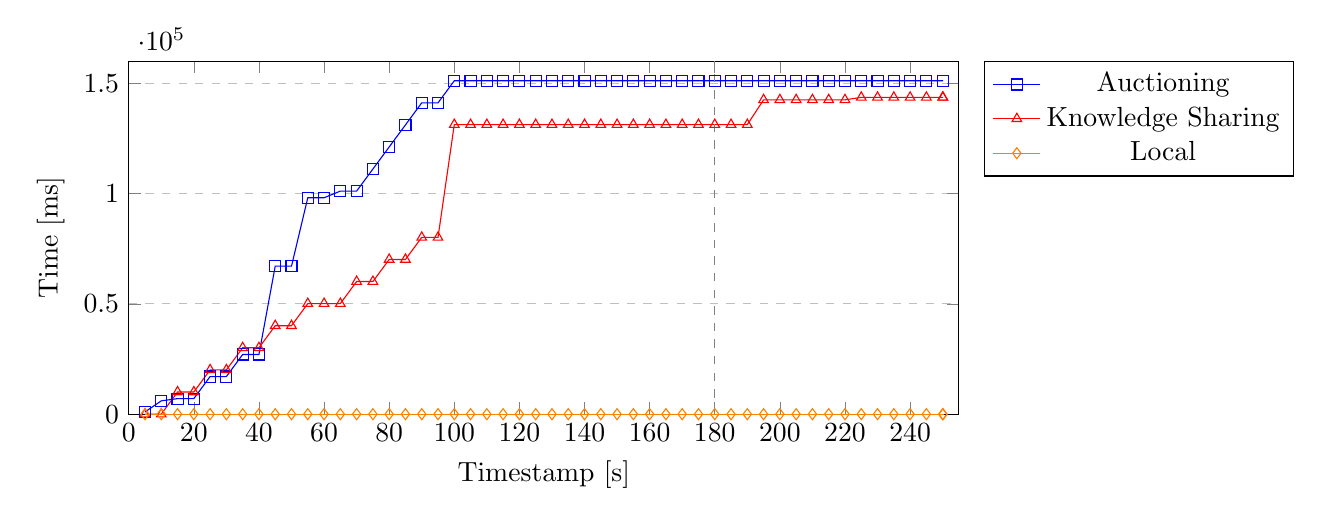
\begin{tikzpicture}
\begin{axis}[
    xlabel={Timestamp [s]},
    ylabel={Time [ms]},
    xmin=0, xmax=255000,
    ymin=0, ymax=160016,
    legend pos=outer north east,
    ymajorgrids=true,
    grid style=dashed,
    width=\textwidth,
    height=0.5\textwidth,
    scaled x ticks=base 10:-3,
    xtick scale label code/.code={}
]

	\addplot[color=blue,mark=square] coordinates {
        (5000,1002)(10000,6043)(15000,7052)(20000,7052)(25000,17062)(30000,17062)(35000,27073)(40000,27073)(45000,67114)(50000,67114)(55000,98143)(60000,98143)(65000,101166)(70000,101166)(75000,111175)(80000,121177)(85000,131184)(90000,141191)(95000,141191)(100000,151201)(105000,151201)(110000,151201)(115000,151201)(120000,151201)(125000,151201)(130000,151201)(135000,151201)(140000,151201)(145000,151201)(150000,151201)(155000,151201)(160000,151201)(165000,151201)(170000,151201)(175000,151201)(180000,151201)(185000,151201)(190000,151201)(195000,151201)(200000,151201)(205000,151201)(210000,151201)(215000,151201)(220000,151201)(225000,151201)(230000,151201)(235000,151201)(240000,151201)(245000,151201)(250000,151201)(250139,151201)
    };
    \addlegendentry{Auctioning}
	\addplot[color=red,mark=triangle] coordinates {
        (5000,0)(10000,0)(15000,10047)(20000,10047)(25000,20080)(30000,20080)(35000,30102)(40000,30102)(45000,40126)(50000,40126)(55000,50144)(60000,50144)(65000,50144)(70000,60152)(75000,60152)(80000,70161)(85000,70161)(90000,80163)(95000,80163)(100000,131322)(105000,131322)(110000,131322)(115000,131322)(120000,131322)(125000,131322)(130000,131322)(135000,131322)(140000,131322)(145000,131322)(150000,131322)(155000,131322)(160000,131322)(165000,131322)(170000,131322)(175000,131322)(180000,131322)(185000,131322)(190000,131322)(195000,142557)(200000,142557)(205000,142557)(210000,142557)(215000,142557)(220000,142557)(225000,143673)(230000,143673)(235000,143673)(240000,143673)(245000,143673)(250000,143673)(250111,143673)
    };
    \addlegendentry{Knowledge Sharing}
	\addplot[color=orange,mark=diamond] coordinates {
        (5000,0)(10000,0)(15000,0)(20000,0)(25000,0)(30000,0)(35000,0)(40000,0)(45000,0)(50000,0)(55000,0)(60000,0)(65000,0)(70000,0)(75000,0)(80000,0)(85000,0)(90000,0)(95000,0)(100000,0)(105000,0)(110000,0)(115000,0)(120000,0)(125000,0)(130000,0)(135000,0)(140000,0)(145000,0)(150000,0)(155000,0)(160000,0)(165000,0)(170000,0)(175000,0)(180000,0)(185000,0)(190000,0)(195000,0)(200000,0)(205000,0)(210000,0)(215000,0)(220000,0)(225000,0)(230000,0)(235000,0)(240000,0)(245000,0)(250000,0)(250115,0)
    };
    \addlegendentry{Local}

	\addplot[color=gray, dashed,] coordinates {(180000,0) (180000,160016)};


\end{axis}
\end{tikzpicture}
    \caption{Graph showing the sum of time spent adapting by agents in the risk introduction scenario.}
\end{figure}

\subsection{Scenario 3: Growing Infrastructure}
\begin{figure}[H]
    \centering
    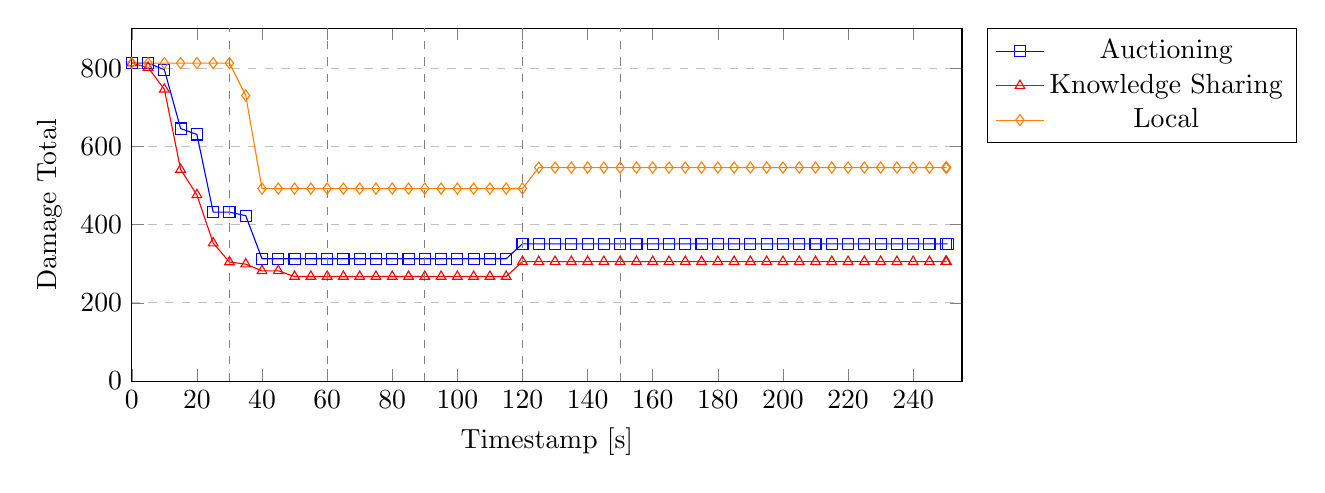
\begin{tikzpicture}
\begin{axis}[
    xlabel={Timestamp [s]},
    ylabel={Damage Total},
    xmin=0, xmax=255000,
    ymin=0, ymax=902,
    legend pos=outer north east,
    ymajorgrids=true,
    grid style=dashed,
    width=\textwidth,
    height=0.5\textwidth,
    scaled x ticks=base 10:-3,
    xtick scale label code/.code={}
]

	\addplot[color=blue,mark=square] coordinates {
        (0,812.71)(5000,812.71)(10000,796.17)(15000,645.46)(20000,630.54)(25000,431.97)(30000,431.97)(35000,422.77)(40000,312.76)(45000,312.76)(50000,312.76)(55000,312.76)(60000,312.76)(65000,312.76)(70000,312.76)(75000,312.76)(80000,312.76)(85000,312.76)(90000,312.76)(95000,312.76)(100000,312.76)(105000,312.76)(110000,312.76)(115000,312.76)(120000,350.90)(125000,350.90)(130000,350.90)(135000,350.90)(140000,350.90)(145000,350.90)(150000,350.90)(155000,350.90)(160000,350.90)(165000,350.90)(170000,350.90)(175000,350.90)(180000,350.90)(185000,350.90)(190000,350.90)(195000,350.90)(200000,350.90)(205000,350.90)(210000,350.90)(215000,350.90)(220000,350.90)(225000,350.90)(230000,350.90)(235000,350.90)(240000,350.90)(245000,350.90)(250000,350.90)(250569,350.90)
    };
    \addlegendentry{Auctioning}
	\addplot[color=red,mark=triangle] coordinates {
        (0,812.71)(5000,801.69)(10000,745.99)(15000,541.01)(20000,476.06)(25000,352.72)(30000,304.33)(35000,298.99)(40000,281.89)(45000,281.89)(50000,267.31)(55000,267.31)(60000,267.31)(65000,267.31)(70000,267.31)(75000,267.31)(80000,267.31)(85000,267.31)(90000,267.31)(95000,267.31)(100000,267.31)(105000,267.31)(110000,267.31)(115000,267.31)(120000,305.45)(125000,305.45)(130000,305.45)(135000,305.45)(140000,305.45)(145000,305.45)(150000,305.45)(155000,305.45)(160000,305.45)(165000,305.45)(170000,305.45)(175000,305.45)(180000,305.45)(185000,305.45)(190000,305.45)(195000,305.45)(200000,305.45)(205000,305.45)(210000,305.45)(215000,305.45)(220000,305.45)(225000,305.45)(230000,305.45)(235000,305.45)(240000,305.45)(245000,305.45)(250000,305.45)(250242,305.45)
    };
    \addlegendentry{Knowledge Sharing}
	\addplot[color=orange,mark=diamond] coordinates {
        (0,812.71)(5000,812.71)(10000,812.71)(15000,812.71)(20000,812.71)(25000,812.71)(30000,812.71)(35000,729.98)(40000,492.04)(45000,492.04)(50000,492.04)(55000,492.04)(60000,492.04)(65000,492.04)(70000,492.04)(75000,492.04)(80000,492.04)(85000,492.04)(90000,492.04)(95000,492.04)(100000,492.04)(105000,492.04)(110000,492.04)(115000,492.04)(120000,492.04)(125000,545.78)(130000,545.78)(135000,545.78)(140000,545.78)(145000,545.78)(150000,545.78)(155000,545.78)(160000,545.78)(165000,545.78)(170000,545.78)(175000,545.78)(180000,545.78)(185000,545.78)(190000,545.78)(195000,545.78)(200000,545.78)(205000,545.78)(210000,545.78)(215000,545.78)(220000,545.78)(225000,545.78)(230000,545.78)(235000,545.78)(240000,545.78)(245000,545.78)(250000,545.78)(250282,545.78)
    };
    \addlegendentry{Local}

	\addplot[color=gray, dashed,] coordinates {(30000,0) (30000,902)};
	\addplot[color=gray, dashed,] coordinates {(60000,0) (60000,902)};
	\addplot[color=gray, dashed,] coordinates {(90000,0) (90000,902)};
	\addplot[color=gray, dashed,] coordinates {(120000,0) (120000,902)};
	\addplot[color=gray, dashed,] coordinates {(150000,0) (150000,902)};


\end{axis}
\end{tikzpicture}
    \caption{This graph shows the overall damage of the system in the growing scenario. The damage is shown for each of the three strategies. The vertical lines indicate the time at which a node is introduced.}
    \label{fig:overall-damage-growing}
\end{figure}


\begin{figure}[H]
    \centering
    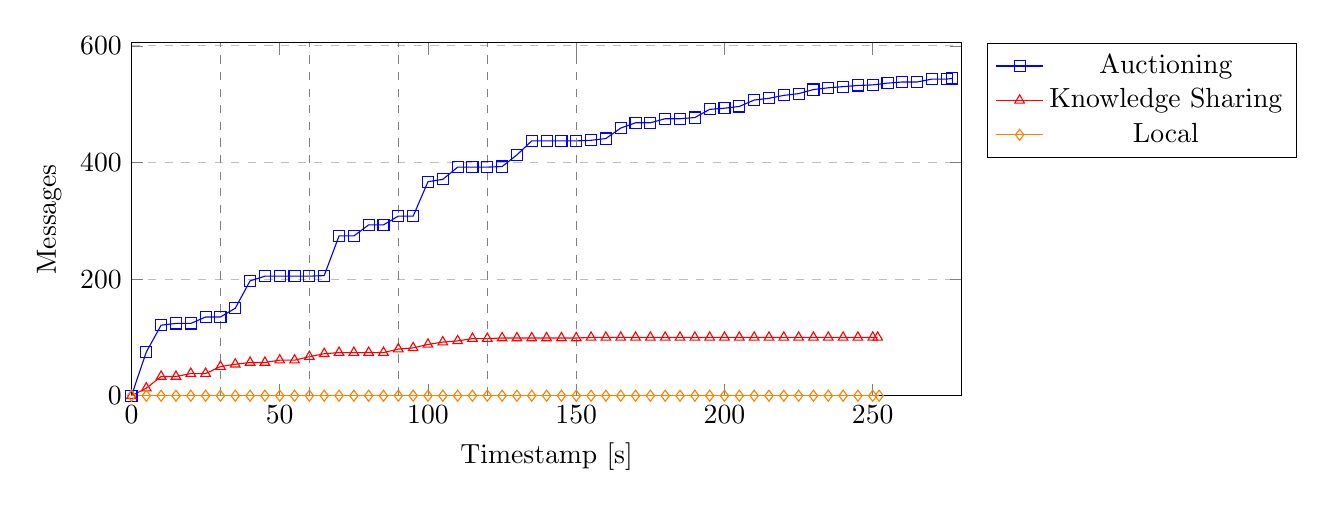
\begin{tikzpicture}
\begin{axis}[
    xlabel={Timestamp [s]},
    ylabel={Messages},
    xmin=0, xmax=280000,
    ymin=0, ymax=605,
    legend pos=outer north east,
    ymajorgrids=true,
    grid style=dashed,
    width=\textwidth,
    height=0.5\textwidth,
    scaled x ticks=base 10:-3,
    xtick scale label code/.code={}
]

	\addplot[color=blue,mark=square] coordinates {
        (0,0)(5000,75)(10000,121)(15000,124)(20000,124)(25000,135)(30000,135)(35000,150)(40000,197)(45000,205)(50000,205)(55000,205)(60000,205)(65000,206)(70000,274)(75000,274)(80000,293)(85000,293)(90000,308)(95000,308)(100000,367)(105000,371)(110000,392)(115000,392)(120000,392)(125000,393)(130000,413)(135000,437)(140000,437)(145000,437)(150000,437)(155000,438)(160000,441)(165000,459)(170000,468)(175000,468)(180000,475)(185000,475)(190000,477)(195000,491)(200000,493)(205000,496)(210000,507)(215000,510)(220000,515)(225000,518)(230000,525)(235000,528)(240000,530)(245000,532)(250000,533)(255000,536)(260000,538)(265000,538)(270000,543)(275000,543)(276704,544)
    };
    \addlegendentry{Auctioning}
	\addplot[color=red,mark=triangle] coordinates {
        (0,0)(5000,13)(10000,33)(15000,33)(20000,38)(25000,38)(30000,50)(35000,54)(40000,57)(45000,57)(50000,61)(55000,61)(60000,67)(65000,72)(70000,74)(75000,74)(80000,74)(85000,74)(90000,80)(95000,82)(100000,88)(105000,92)(110000,94)(115000,98)(120000,98)(125000,99)(130000,99)(135000,99)(140000,99)(145000,99)(150000,99)(155000,100)(160000,100)(165000,100)(170000,100)(175000,100)(180000,100)(185000,100)(190000,100)(195000,100)(200000,100)(205000,100)(210000,100)(215000,100)(220000,100)(225000,100)(230000,100)(235000,100)(240000,100)(245000,100)(250000,100)(251678,100)
    };
    \addlegendentry{Knowledge Sharing}
	\addplot[color=orange,mark=diamond] coordinates {
        (0,0)(5000,0)(10000,0)(15000,0)(20000,0)(25000,0)(30000,0)(35000,0)(40000,0)(45000,0)(50000,0)(55000,0)(60000,0)(65000,0)(70000,0)(75000,0)(80000,0)(85000,0)(90000,0)(95000,0)(100000,0)(105000,0)(110000,0)(115000,0)(120000,0)(125000,0)(130000,0)(135000,0)(140000,0)(145000,0)(150000,0)(155000,0)(160000,0)(165000,0)(170000,0)(175000,0)(180000,0)(185000,0)(190000,0)(195000,0)(200000,0)(205000,0)(210000,0)(215000,0)(220000,0)(225000,0)(230000,0)(235000,0)(240000,0)(245000,0)(250000,0)(252143,0)
    };
    \addlegendentry{Local}

	\addplot[color=gray, dashed,] coordinates {(30000,0) (30000,605)};
	\addplot[color=gray, dashed,] coordinates {(60000,0) (60000,605)};
	\addplot[color=gray, dashed,] coordinates {(90000,0) (90000,605)};
	\addplot[color=gray, dashed,] coordinates {(120000,0) (120000,605)};
	\addplot[color=gray, dashed,] coordinates {(150000,0) (150000,605)};


\end{axis}
\end{tikzpicture}
    \caption{Graph showing the total amount of messages sent between agents in the growing infrastructure scenario.}
\end{figure}
\begin{figure}[H]
    \centering
    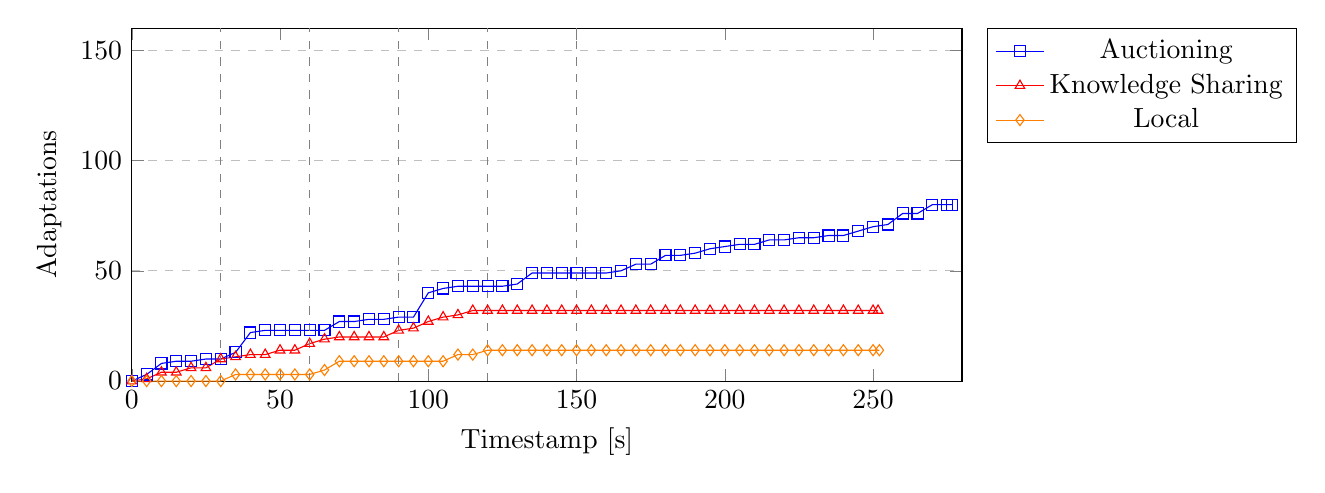
\begin{tikzpicture}
\begin{axis}[
    xlabel={Timestamp [s]},
    ylabel={Adaptations},
    xmin=0, xmax=280000,
    ymin=0, ymax=160,
    legend pos=outer north east,
    ymajorgrids=true,
    grid style=dashed,
    width=\textwidth,
    height=0.5\textwidth,
    scaled x ticks=base 10:-3,
    xtick scale label code/.code={}
]

	\addplot[color=blue,mark=square] coordinates {
        (0,0)(5000,3)(10000,8)(15000,9)(20000,9)(25000,10)(30000,10)(35000,13)(40000,22)(45000,23)(50000,23)(55000,23)(60000,23)(65000,23)(70000,27)(75000,27)(80000,28)(85000,28)(90000,29)(95000,29)(100000,40)(105000,42)(110000,43)(115000,43)(120000,43)(125000,43)(130000,44)(135000,49)(140000,49)(145000,49)(150000,49)(155000,49)(160000,49)(165000,50)(170000,53)(175000,53)(180000,57)(185000,57)(190000,58)(195000,60)(200000,61)(205000,62)(210000,62)(215000,64)(220000,64)(225000,65)(230000,65)(235000,66)(240000,66)(245000,68)(250000,70)(255000,71)(260000,76)(265000,76)(270000,80)(275000,80)(276704,80)
    };
    \addlegendentry{Auctioning}
	\addplot[color=red,mark=triangle] coordinates {
        (0,0)(5000,1)(10000,4)(15000,4)(20000,6)(25000,6)(30000,10)(35000,11)(40000,12)(45000,12)(50000,14)(55000,14)(60000,17)(65000,19)(70000,20)(75000,20)(80000,20)(85000,20)(90000,23)(95000,24)(100000,27)(105000,29)(110000,30)(115000,32)(120000,32)(125000,32)(130000,32)(135000,32)(140000,32)(145000,32)(150000,32)(155000,32)(160000,32)(165000,32)(170000,32)(175000,32)(180000,32)(185000,32)(190000,32)(195000,32)(200000,32)(205000,32)(210000,32)(215000,32)(220000,32)(225000,32)(230000,32)(235000,32)(240000,32)(245000,32)(250000,32)(251678,32)
    };
    \addlegendentry{Knowledge Sharing}
	\addplot[color=orange,mark=diamond] coordinates {
        (0,0)(5000,0)(10000,0)(15000,0)(20000,0)(25000,0)(30000,0)(35000,3)(40000,3)(45000,3)(50000,3)(55000,3)(60000,3)(65000,5)(70000,9)(75000,9)(80000,9)(85000,9)(90000,9)(95000,9)(100000,9)(105000,9)(110000,12)(115000,12)(120000,14)(125000,14)(130000,14)(135000,14)(140000,14)(145000,14)(150000,14)(155000,14)(160000,14)(165000,14)(170000,14)(175000,14)(180000,14)(185000,14)(190000,14)(195000,14)(200000,14)(205000,14)(210000,14)(215000,14)(220000,14)(225000,14)(230000,14)(235000,14)(240000,14)(245000,14)(250000,14)(252143,14)
    };
    \addlegendentry{Local}

	\addplot[color=gray, dashed,] coordinates {(30000,0) (30000,160)};
	\addplot[color=gray, dashed,] coordinates {(60000,0) (60000,160)};
	\addplot[color=gray, dashed,] coordinates {(90000,0) (90000,160)};
	\addplot[color=gray, dashed,] coordinates {(120000,0) (120000,160)};
	\addplot[color=gray, dashed,] coordinates {(150000,0) (150000,160)};


\end{axis}
\end{tikzpicture}
    \caption{Graph showing the total amount of adaptations applied by agents in the growing scenario.}
\end{figure}
\begin{figure}[H]
    \centering
        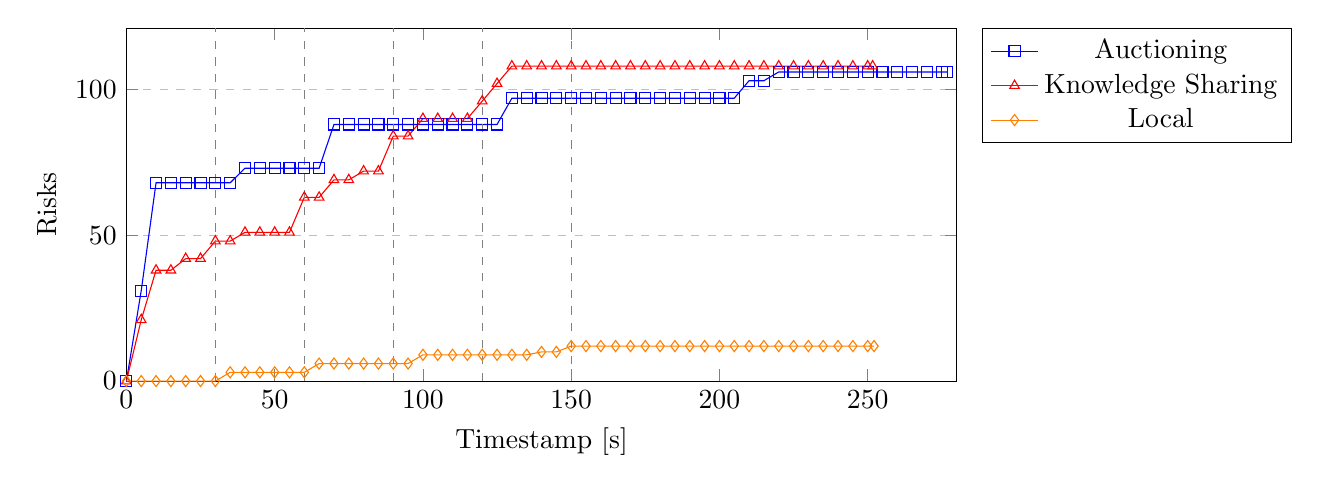
\begin{tikzpicture}
\begin{axis}[
    xlabel={Timestamp [s]},
    ylabel={Risks},
    xmin=0, xmax=280000,
    ymin=0, ymax=121,
    legend pos=outer north east,
    ymajorgrids=true,
    grid style=dashed,
    width=\textwidth,
    height=0.5\textwidth,
    scaled x ticks=base 10:-3,
    xtick scale label code/.code={}
]

	\addplot[color=blue,mark=square] coordinates {
        (0,0)(5000,31)(10000,68)(15000,68)(20000,68)(25000,68)(30000,68)(35000,68)(40000,73)(45000,73)(50000,73)(55000,73)(60000,73)(65000,73)(70000,88)(75000,88)(80000,88)(85000,88)(90000,88)(95000,88)(100000,88)(105000,88)(110000,88)(115000,88)(120000,88)(125000,88)(130000,97)(135000,97)(140000,97)(145000,97)(150000,97)(155000,97)(160000,97)(165000,97)(170000,97)(175000,97)(180000,97)(185000,97)(190000,97)(195000,97)(200000,97)(205000,97)(210000,103)(215000,103)(220000,106)(225000,106)(230000,106)(235000,106)(240000,106)(245000,106)(250000,106)(255000,106)(260000,106)(265000,106)(270000,106)(275000,106)(276704,106)
    };
    \addlegendentry{Auctioning}
	\addplot[color=red,mark=triangle] coordinates {
        (0,0)(5000,21)(10000,38)(15000,38)(20000,42)(25000,42)(30000,48)(35000,48)(40000,51)(45000,51)(50000,51)(55000,51)(60000,63)(65000,63)(70000,69)(75000,69)(80000,72)(85000,72)(90000,84)(95000,84)(100000,90)(105000,90)(110000,90)(115000,90)(120000,96)(125000,102)(130000,108)(135000,108)(140000,108)(145000,108)(150000,108)(155000,108)(160000,108)(165000,108)(170000,108)(175000,108)(180000,108)(185000,108)(190000,108)(195000,108)(200000,108)(205000,108)(210000,108)(215000,108)(220000,108)(225000,108)(230000,108)(235000,108)(240000,108)(245000,108)(250000,108)(251678,108)
    };
    \addlegendentry{Knowledge Sharing}
	\addplot[color=orange,mark=diamond] coordinates {
        (0,0)(5000,0)(10000,0)(15000,0)(20000,0)(25000,0)(30000,0)(35000,3)(40000,3)(45000,3)(50000,3)(55000,3)(60000,3)(65000,6)(70000,6)(75000,6)(80000,6)(85000,6)(90000,6)(95000,6)(100000,9)(105000,9)(110000,9)(115000,9)(120000,9)(125000,9)(130000,9)(135000,9)(140000,10)(145000,10)(150000,12)(155000,12)(160000,12)(165000,12)(170000,12)(175000,12)(180000,12)(185000,12)(190000,12)(195000,12)(200000,12)(205000,12)(210000,12)(215000,12)(220000,12)(225000,12)(230000,12)(235000,12)(240000,12)(245000,12)(250000,12)(252143,12)
    };
    \addlegendentry{Local}

	\addplot[color=gray, dashed,] coordinates {(30000,0) (30000,121)};
	\addplot[color=gray, dashed,] coordinates {(60000,0) (60000,121)};
	\addplot[color=gray, dashed,] coordinates {(90000,0) (90000,121)};
	\addplot[color=gray, dashed,] coordinates {(120000,0) (120000,121)};
	\addplot[color=gray, dashed,] coordinates {(150000,0) (150000,121)};


\end{axis}
\end{tikzpicture}
    \caption{Graph showing the number of unique risks detected by agents in the growing scenario.}
\end{figure}
\begin{figure}[H]
    \centering
        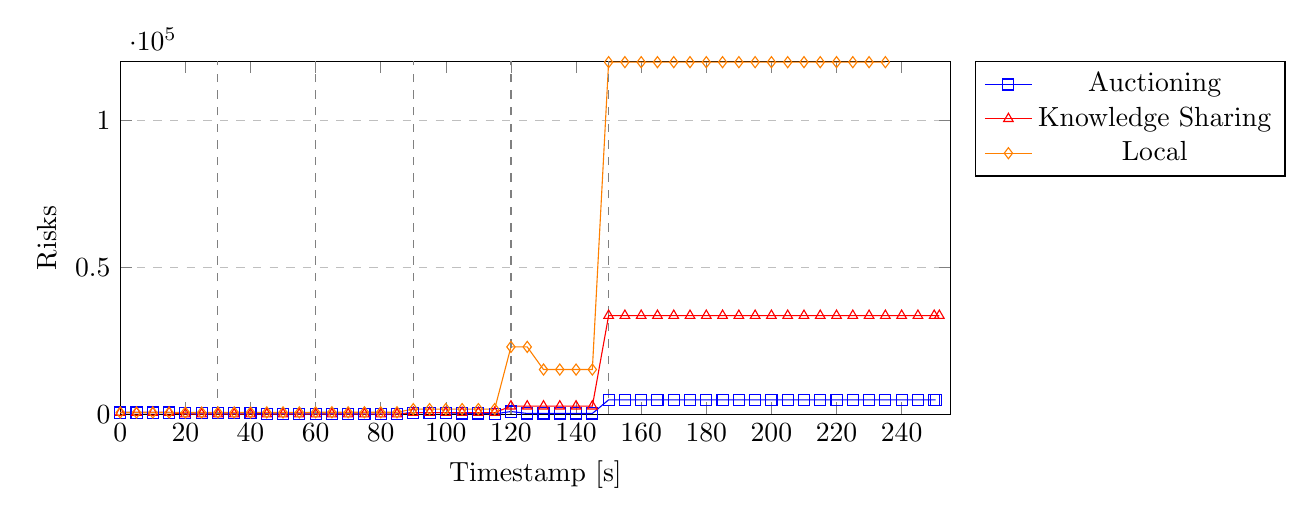
\begin{tikzpicture}
\begin{axis}[
    xlabel={Timestamp [s]},
    ylabel={Risks},
    xmin=0, xmax=255000,
    ymin=0, ymax=120012,
    legend pos=outer north east,
    ymajorgrids=true,
    grid style=dashed,
    width=\textwidth,
    height=0.5\textwidth,
    scaled x ticks=base 10:-3,
    xtick scale label code/.code={}
]

	\addplot[color=blue,mark=square] coordinates {
        (0,563)(5000,563)(10000,563)(15000,563)(20000,360)(25000,360)(30000,399)(35000,399)(40000,399)(45000,100)(50000,100)(55000,60)(60000,80)(65000,80)(70000,80)(75000,40)(80000,40)(85000,40)(90000,520)(95000,520)(100000,520)(105000,240)(110000,240)(115000,100)(120000,900)(125000,240)(130000,240)(135000,240)(140000,240)(145000,240)(150000,4880)(155000,4880)(160000,4880)(165000,4880)(170000,4880)(175000,4880)(180000,4880)(185000,4880)(190000,4880)(195000,4880)(200000,4880)(205000,4880)(210000,4880)(215000,4880)(220000,4880)(225000,4880)(230000,4880)(235000,4880)(240000,4880)(245000,4880)(250000,4880)(250452,4880)
    };
    \addlegendentry{Auctioning}
	\addplot[color=red,mark=triangle] coordinates {
        (0,563)(5000,563)(10000,563)(15000,563)(20000,10)(25000,10)(30000,40)(35000,20)(40000,20)(45000,20)(50000,20)(55000,20)(60000,40)(65000,40)(70000,40)(75000,40)(80000,40)(85000,40)(90000,520)(95000,520)(100000,520)(105000,520)(110000,520)(115000,520)(120000,2720)(125000,2720)(130000,2720)(135000,2720)(140000,2720)(145000,2720)(150000,33540)(155000,33540)(160000,33540)(165000,33540)(170000,33540)(175000,33540)(180000,33540)(185000,33540)(190000,33540)(195000,33540)(200000,33540)(205000,33540)(210000,33540)(215000,33540)(220000,33540)(225000,33540)(230000,33540)(235000,33540)(240000,33540)(245000,33540)(250000,33540)(251574,33540)
    };
    \addlegendentry{Knowledge Sharing}
	\addplot[color=orange,mark=diamond] coordinates {
        (0,563)(5000,563)(10000,563)(15000,563)(20000,563)(25000,563)(30000,608)(35000,608)(40000,608)(45000,608)(50000,608)(55000,608)(60000,653)(65000,653)(70000,653)(75000,653)(80000,653)(85000,653)(90000,1733)(95000,1733)(100000,1733)(105000,1733)(110000,1733)(115000,1733)(120000,22883)(125000,22883)(130000,15180)(135000,15180)(140000,15180)(145000,15180)(150000,119730)(155000,119730)(160000,119730)(165000,119730)(170000,119730)(175000,119730)(180000,119730)(185000,119730)(190000,119730)(195000,119730)(200000,119730)(205000,119730)(210000,119730)(215000,119730)(220000,119730)(225000,119730)(230000,119730)(235000,119730)
    };
    \addlegendentry{Local}

	\addplot[color=gray, dashed,] coordinates {(30000,0) (30000,120012)};
	\addplot[color=gray, dashed,] coordinates {(60000,0) (60000,120012)};
	\addplot[color=gray, dashed,] coordinates {(90000,0) (90000,120012)};
	\addplot[color=gray, dashed,] coordinates {(120000,0) (120000,120012)};
	\addplot[color=gray, dashed,] coordinates {(150000,0) (150000,120012)};


\end{axis}
\end{tikzpicture}
    \caption{Graph showing the number of remaining risks in the infrastructure in the growing scenario.}
\end{figure}
\begin{figure}[H]
    \centering
        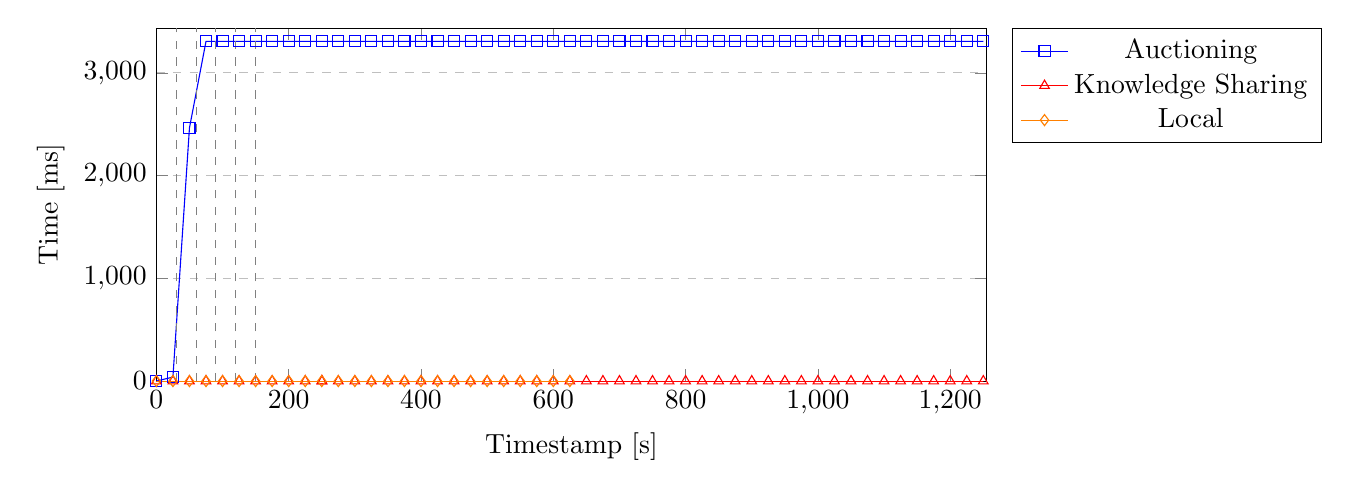
\begin{tikzpicture}
\begin{axis}[
    xlabel={Timestamp [s]},
    ylabel={Time [ms]},
    xmin=0, xmax=1255000,
    ymin=0, ymax=3434,
    legend pos=outer north east,
    ymajorgrids=true,
    grid style=dashed,
    width=\textwidth,
    height=0.5\textwidth,
    scaled x ticks=base 10:-3,
    xtick scale label code/.code={}
]

	\addplot[color=blue,mark=square] coordinates {
        (0,0)(25000,39)(50000,2464)(75000,3306)(100000,3306)(125000,3306)(150000,3306)(175000,3306)(200000,3306)(225000,3306)(250000,3306)(275000,3306)(300000,3306)(325000,3306)(350000,3306)(375000,3306)(400000,3306)(425000,3306)(450000,3306)(475000,3306)(500000,3306)(525000,3306)(550000,3306)(575000,3306)(600000,3306)(625000,3306)(650000,3306)(675000,3306)(700000,3306)(725000,3306)(750000,3306)(775000,3306)(800000,3306)(825000,3306)(850000,3306)(875000,3306)(900000,3306)(925000,3306)(950000,3306)(975000,3306)(1000000,3306)(1025000,3306)(1050000,3306)(1075000,3306)(1100000,3306)(1125000,3306)(1150000,3306)(1175000,3306)(1200000,3306)(1225000,3306)(1250000,3306)(250447,3306)
    };
    \addlegendentry{Auctioning}
	\addplot[color=red,mark=triangle] coordinates {
        (0,0)(25000,0)(50000,0)(75000,0)(100000,0)(125000,0)(150000,0)(175000,0)(200000,0)(225000,0)(250000,0)(275000,0)(300000,0)(325000,0)(350000,0)(375000,0)(400000,0)(425000,0)(450000,0)(475000,0)(500000,0)(525000,0)(550000,0)(575000,0)(600000,0)(625000,0)(650000,0)(675000,0)(700000,0)(725000,0)(750000,0)(775000,0)(800000,0)(825000,0)(850000,0)(875000,0)(900000,0)(925000,0)(950000,0)(975000,0)(1000000,0)(1025000,0)(1050000,0)(1075000,0)(1100000,0)(1125000,0)(1150000,0)(1175000,0)(1200000,0)(1225000,0)(1250000,0)(250418,0)
    };
    \addlegendentry{Knowledge Sharing}
	\addplot[color=orange,mark=diamond] coordinates {
        (0,0)(25000,0)(50000,0)(75000,0)(100000,0)(125000,0)(150000,0)(175000,0)(200000,0)(225000,0)(250000,0)(275000,0)(300000,0)(325000,0)(350000,0)(375000,0)(400000,0)(425000,0)(450000,0)(475000,0)(500000,0)(525000,0)(550000,0)(575000,0)(600000,0)(625000,0)
    };
    \addlegendentry{Local}

	\addplot[color=gray, dashed,] coordinates {(30000,0) (30000,3434)};
	\addplot[color=gray, dashed,] coordinates {(60000,0) (60000,3434)};
	\addplot[color=gray, dashed,] coordinates {(90000,0) (90000,3434)};
	\addplot[color=gray, dashed,] coordinates {(120000,0) (120000,3434)};
	\addplot[color=gray, dashed,] coordinates {(150000,0) (150000,3434)};


\end{axis}
\end{tikzpicture}
    \caption{Graph showing the sum of time spent auctioning by agents in the growing scenario.}
\end{figure}
\begin{figure}[H]
    \centering
        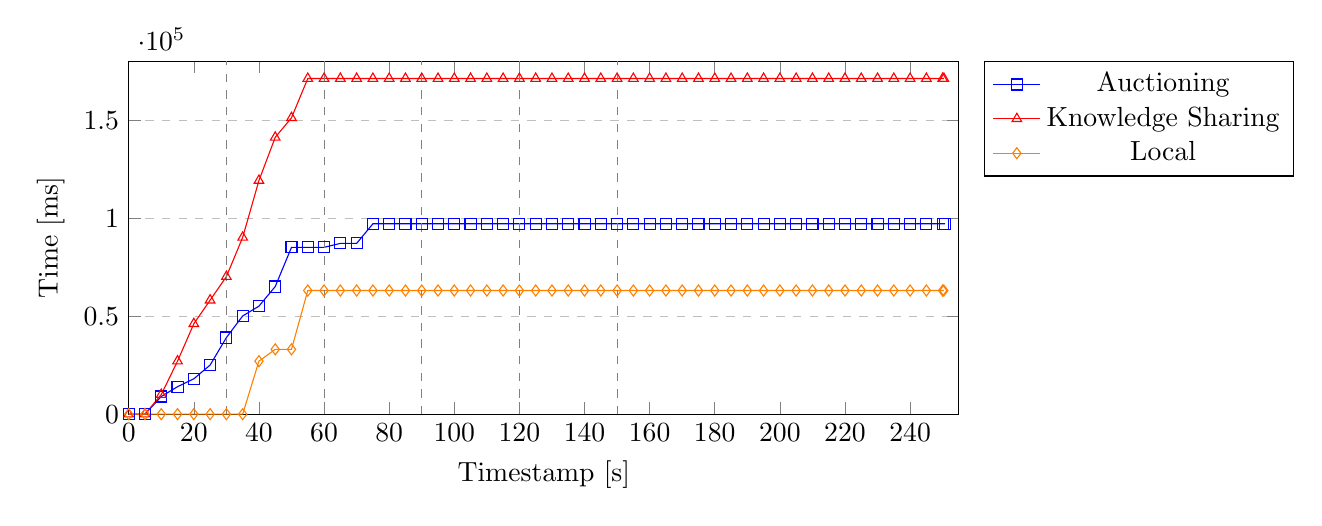
\begin{tikzpicture}
\begin{axis}[
    xlabel={Timestamp [s]},
    ylabel={Time [ms]},
    xmin=0, xmax=255000,
    ymin=0, ymax=180018,
    legend pos=outer north east,
    ymajorgrids=true,
    grid style=dashed,
    width=\textwidth,
    height=0.5\textwidth,
    scaled x ticks=base 10:-3,
    xtick scale label code/.code={}
]

	\addplot[color=blue,mark=square] coordinates {
        (0,0)(5000,0)(10000,9022)(15000,14028)(20000,18038)(25000,25054)(30000,39076)(35000,50106)(40000,55112)(45000,65114)(50000,85122)(55000,85122)(60000,85122)(65000,87124)(70000,87124)(75000,97131)(80000,97131)(85000,97131)(90000,97131)(95000,97131)(100000,97131)(105000,97131)(110000,97131)(115000,97131)(120000,97131)(125000,97131)(130000,97131)(135000,97131)(140000,97131)(145000,97131)(150000,97131)(155000,97131)(160000,97131)(165000,97131)(170000,97131)(175000,97131)(180000,97131)(185000,97131)(190000,97131)(195000,97131)(200000,97131)(205000,97131)(210000,97131)(215000,97131)(220000,97131)(225000,97131)(230000,97131)(235000,97131)(240000,97131)(245000,97131)(250000,97131)(250721,97131)
    };
    \addlegendentry{Auctioning}
	\addplot[color=red,mark=triangle] coordinates {
        (0,0)(5000,0)(10000,10020)(15000,27063)(20000,46118)(25000,58158)(30000,70170)(35000,90181)(40000,119203)(45000,141218)(50000,151223)(55000,171237)(60000,171237)(65000,171237)(70000,171237)(75000,171237)(80000,171237)(85000,171237)(90000,171237)(95000,171237)(100000,171237)(105000,171237)(110000,171237)(115000,171237)(120000,171237)(125000,171237)(130000,171237)(135000,171237)(140000,171237)(145000,171237)(150000,171237)(155000,171237)(160000,171237)(165000,171237)(170000,171237)(175000,171237)(180000,171237)(185000,171237)(190000,171237)(195000,171237)(200000,171237)(205000,171237)(210000,171237)(215000,171237)(220000,171237)(225000,171237)(230000,171237)(235000,171237)(240000,171237)(245000,171237)(250000,171237)(250388,171237)
    };
    \addlegendentry{Knowledge Sharing}
	\addplot[color=orange,mark=diamond] coordinates {
        (0,0)(5000,0)(10000,0)(15000,0)(20000,0)(25000,0)(30000,0)(35000,0)(40000,27063)(45000,33082)(50000,33082)(55000,63089)(60000,63089)(65000,63089)(70000,63089)(75000,63089)(80000,63089)(85000,63089)(90000,63089)(95000,63089)(100000,63089)(105000,63089)(110000,63089)(115000,63089)(120000,63089)(125000,63089)(130000,63089)(135000,63089)(140000,63089)(145000,63089)(150000,63089)(155000,63089)(160000,63089)(165000,63089)(170000,63089)(175000,63089)(180000,63089)(185000,63089)(190000,63089)(195000,63089)(200000,63089)(205000,63089)(210000,63089)(215000,63089)(220000,63089)(225000,63089)(230000,63089)(235000,63089)(240000,63089)(245000,63089)(250000,63089)(250358,63089)
    };
    \addlegendentry{Local}

	\addplot[color=gray, dashed,] coordinates {(30000,0) (30000,180018)};
	\addplot[color=gray, dashed,] coordinates {(60000,0) (60000,180018)};
	\addplot[color=gray, dashed,] coordinates {(90000,0) (90000,180018)};
	\addplot[color=gray, dashed,] coordinates {(120000,0) (120000,180018)};
	\addplot[color=gray, dashed,] coordinates {(150000,0) (150000,180018)};


\end{axis}
\end{tikzpicture}
    \caption{Graph showing the sum of time spent adapting by agents in the growing scenario.}
\end{figure}

\subsection{Scenario 4: Unstable Infrastructure}
\begin{figure}[H]
    \centering
    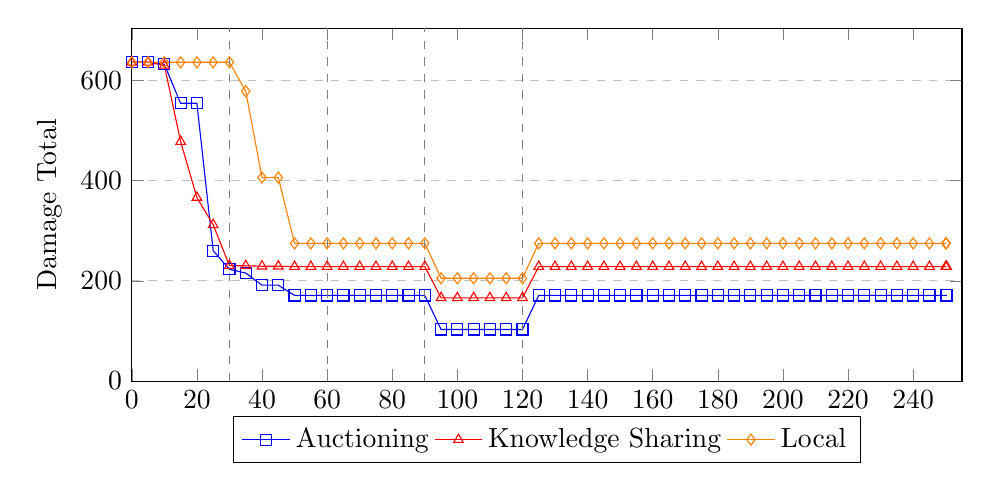
\begin{tikzpicture}
\begin{axis}[
    xlabel={Timestamp [s]},
    ylabel={Damage Total},
    xmin=0, xmax=255000,
    ymin=0, ymax=704,
    legend columns=-1,
    legend style={at={(0.5,-0.1)},anchor=north},
    ymajorgrids=true,
    grid style=dashed,
    width=\textwidth,
    height=0.5\textwidth,
    scaled x ticks=base 10:-3,
    xtick scale label code/.code={}
]

	\addplot[color=blue,mark=square] coordinates {
        (0,636.01)(5000,636.01)(10000,632.06)(15000,554.22)(20000,554.22)(25000,260.13)(30000,223.01)(35000,215.48)(40000,191.39)(45000,191.39)(50000,170.85)(55000,170.85)(60000,170.85)(65000,170.85)(70000,170.85)(75000,170.85)(80000,170.85)(85000,170.85)(90000,170.85)(95000,102.93)(100000,102.93)(105000,102.93)(110000,102.93)(115000,102.93)(120000,102.93)(125000,170.85)(130000,170.85)(135000,170.85)(140000,170.85)(145000,170.85)(150000,170.85)(155000,170.85)(160000,170.85)(165000,170.85)(170000,170.85)(175000,170.85)(180000,170.85)(185000,170.85)(190000,170.85)(195000,170.85)(200000,170.85)(205000,170.85)(210000,170.85)(215000,170.85)(220000,170.85)(225000,170.85)(230000,170.85)(235000,170.85)(240000,170.85)(245000,170.85)(250000,170.85)(250367,170.85)
    };
    \addlegendentry{Auctioning}
	\addplot[color=red,mark=triangle] coordinates {
        (0,636.01)(5000,636.01)(10000,629.93)(15000,477.78)(20000,366.27)(25000,311.79)(30000,230.29)(35000,230.02)(40000,229.15)(45000,229.15)(50000,228.42)(55000,228.42)(60000,228.42)(65000,228.42)(70000,228.42)(75000,228.42)(80000,228.42)(85000,228.42)(90000,228.42)(95000,166.07)(100000,166.07)(105000,166.07)(110000,166.07)(115000,166.07)(120000,166.07)(125000,228.42)(130000,228.42)(135000,228.42)(140000,228.42)(145000,228.42)(150000,228.42)(155000,228.42)(160000,228.42)(165000,228.42)(170000,228.42)(175000,228.42)(180000,228.42)(185000,228.42)(190000,228.42)(195000,228.42)(200000,228.42)(205000,228.42)(210000,228.42)(215000,228.42)(220000,228.42)(225000,228.42)(230000,228.42)(235000,228.42)(240000,228.42)(245000,228.42)(250000,228.42)(250281,228.42)
    };
    \addlegendentry{Knowledge Sharing}
	\addplot[color=orange,mark=diamond] coordinates {
        (0,636.01)(5000,636.01)(10000,636.01)(15000,636.01)(20000,636.01)(25000,636.01)(30000,636.01)(35000,578.19)(40000,406.04)(45000,406.04)(50000,274.81)(55000,274.81)(60000,274.81)(65000,274.81)(70000,274.81)(75000,274.81)(80000,274.81)(85000,274.81)(90000,274.81)(95000,205.14)(100000,205.14)(105000,205.14)(110000,205.14)(115000,205.14)(120000,205.14)(125000,274.81)(130000,274.81)(135000,274.81)(140000,274.81)(145000,274.81)(150000,274.81)(155000,274.81)(160000,274.81)(165000,274.81)(170000,274.81)(175000,274.81)(180000,274.81)(185000,274.81)(190000,274.81)(195000,274.81)(200000,274.81)(205000,274.81)(210000,274.81)(215000,274.81)(220000,274.81)(225000,274.81)(230000,274.81)(235000,274.81)(240000,274.81)(245000,274.81)(250000,274.81)(250187,274.81)
    };
    \addlegendentry{Local}

	\addplot[color=gray, dashed,] coordinates {(30000,0) (30000,704)};
	\addplot[color=gray, dashed,] coordinates {(60000,0) (60000,704)};
	\addplot[color=gray, dashed,] coordinates {(90000,0) (90000,704)};
	\addplot[color=gray, dashed,] coordinates {(120000,0) (120000,704)};


\end{axis}
\end{tikzpicture}
    \caption{This graph shows the overall damage of the system in the unstable scenario. The damage is shown for each of the three strategies. The vertical lines indicate the time at which a node was removed and added again.}
    \label{fig:overall-damage-unstable}
\end{figure}


\begin{figure}[H]
    \centering
    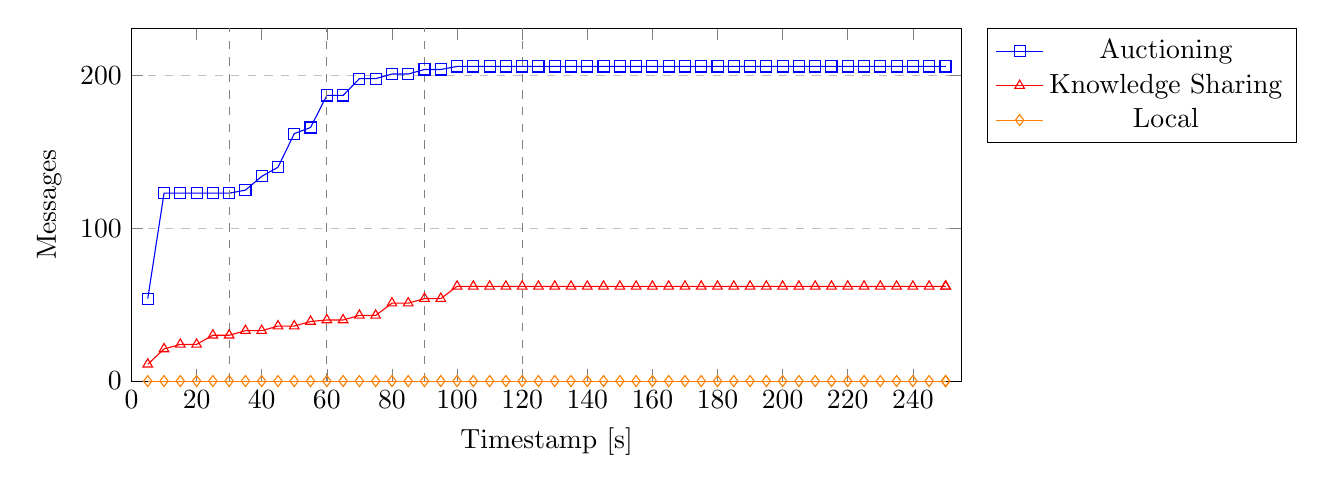
\begin{tikzpicture}
\begin{axis}[
    xlabel={Timestamp [s]},
    ylabel={Messages},
    xmin=0, xmax=255000,
    ymin=0, ymax=231,
    legend pos=outer north east,
    ymajorgrids=true,
    grid style=dashed,
    width=\textwidth,
    height=0.5\textwidth,
    scaled x ticks=base 10:-3,
    xtick scale label code/.code={}
]

	\addplot[color=blue,mark=square] coordinates {
        (5000,54)(10000,123)(15000,123)(20000,123)(25000,123)(30000,123)(35000,125)(40000,134)(45000,140)(50000,162)(55000,166)(60000,187)(65000,187)(70000,198)(75000,198)(80000,201)(85000,201)(90000,204)(95000,204)(100000,206)(105000,206)(110000,206)(115000,206)(120000,206)(125000,206)(130000,206)(135000,206)(140000,206)(145000,206)(150000,206)(155000,206)(160000,206)(165000,206)(170000,206)(175000,206)(180000,206)(185000,206)(190000,206)(195000,206)(200000,206)(205000,206)(210000,206)(215000,206)(220000,206)(225000,206)(230000,206)(235000,206)(240000,206)(245000,206)(250000,206)(250128,206)
    };
    \addlegendentry{Auctioning}
	\addplot[color=red,mark=triangle] coordinates {
        (5000,11)(10000,21)(15000,24)(20000,24)(25000,30)(30000,30)(35000,33)(40000,33)(45000,36)(50000,36)(55000,39)(60000,40)(65000,40)(70000,43)(75000,43)(80000,51)(85000,51)(90000,54)(95000,54)(100000,62)(105000,62)(110000,62)(115000,62)(120000,62)(125000,62)(130000,62)(135000,62)(140000,62)(145000,62)(150000,62)(155000,62)(160000,62)(165000,62)(170000,62)(175000,62)(180000,62)(185000,62)(190000,62)(195000,62)(200000,62)(205000,62)(210000,62)(215000,62)(220000,62)(225000,62)(230000,62)(235000,62)(240000,62)(245000,62)(250000,62)(250118,62)
    };
    \addlegendentry{Knowledge Sharing}
	\addplot[color=orange,mark=diamond] coordinates {
        (5000,0)(10000,0)(15000,0)(20000,0)(25000,0)(30000,0)(35000,0)(40000,0)(45000,0)(50000,0)(55000,0)(60000,0)(65000,0)(70000,0)(75000,0)(80000,0)(85000,0)(90000,0)(95000,0)(100000,0)(105000,0)(110000,0)(115000,0)(120000,0)(125000,0)(130000,0)(135000,0)(140000,0)(145000,0)(150000,0)(155000,0)(160000,0)(165000,0)(170000,0)(175000,0)(180000,0)(185000,0)(190000,0)(195000,0)(200000,0)(205000,0)(210000,0)(215000,0)(220000,0)(225000,0)(230000,0)(235000,0)(240000,0)(245000,0)(250000,0)(250107,0)
    };
    \addlegendentry{Local}

	\addplot[color=gray, dashed,] coordinates {(30000,0) (30000,231)};
	\addplot[color=gray, dashed,] coordinates {(60000,0) (60000,231)};
	\addplot[color=gray, dashed,] coordinates {(90000,0) (90000,231)};
	\addplot[color=gray, dashed,] coordinates {(120000,0) (120000,231)};


\end{axis}
\end{tikzpicture}
    \caption{Graph showing the total amount of messages sent between agents in the unstable scenario.}
\end{figure}
\begin{figure}[H]
    \centering
    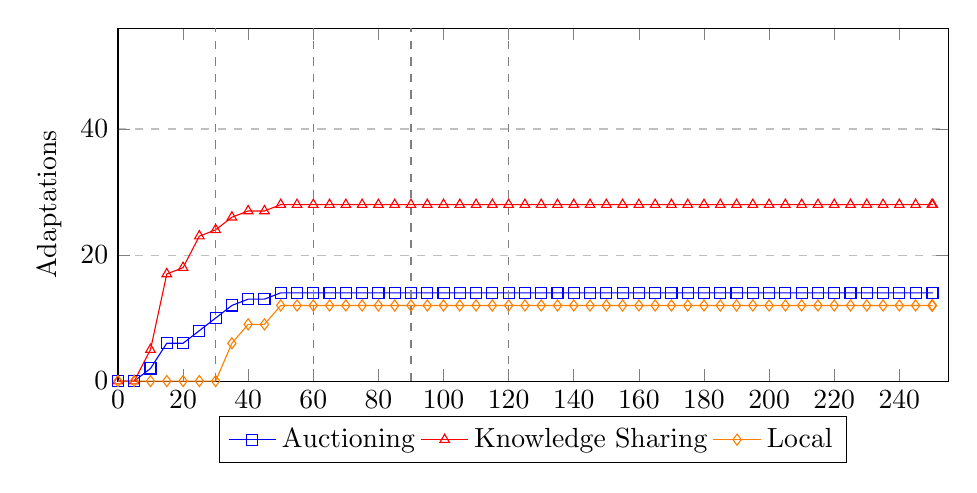
\begin{tikzpicture}
\begin{axis}[
    xlabel={Timestamp [s]},
    ylabel={Adaptations},
    xmin=0, xmax=255000,
    ymin=0, ymax=56,
    legend columns=-1,
    legend style={at={(0.5,-0.1)},anchor=north},
    ymajorgrids=true,
    grid style=dashed,
    width=\textwidth,
    height=0.5\textwidth,
    scaled x ticks=base 10:-3,
    xtick scale label code/.code={}
]

	\addplot[color=blue,mark=square] coordinates {
        (0,0)(5000,0)(10000,2)(15000,6)(20000,6)(25000,8)(30000,10)(35000,12)(40000,13)(45000,13)(50000,14)(55000,14)(60000,14)(65000,14)(70000,14)(75000,14)(80000,14)(85000,14)(90000,14)(95000,14)(100000,14)(105000,14)(110000,14)(115000,14)(120000,14)(125000,14)(130000,14)(135000,14)(140000,14)(145000,14)(150000,14)(155000,14)(160000,14)(165000,14)(170000,14)(175000,14)(180000,14)(185000,14)(190000,14)(195000,14)(200000,14)(205000,14)(210000,14)(215000,14)(220000,14)(225000,14)(230000,14)(235000,14)(240000,14)(245000,14)(250000,14)(250367,14)
    };
    \addlegendentry{Auctioning}
	\addplot[color=red,mark=triangle] coordinates {
        (0,0)(5000,0)(10000,5)(15000,17)(20000,18)(25000,23)(30000,24)(35000,26)(40000,27)(45000,27)(50000,28)(55000,28)(60000,28)(65000,28)(70000,28)(75000,28)(80000,28)(85000,28)(90000,28)(95000,28)(100000,28)(105000,28)(110000,28)(115000,28)(120000,28)(125000,28)(130000,28)(135000,28)(140000,28)(145000,28)(150000,28)(155000,28)(160000,28)(165000,28)(170000,28)(175000,28)(180000,28)(185000,28)(190000,28)(195000,28)(200000,28)(205000,28)(210000,28)(215000,28)(220000,28)(225000,28)(230000,28)(235000,28)(240000,28)(245000,28)(250000,28)(250281,28)
    };
    \addlegendentry{Knowledge Sharing}
	\addplot[color=orange,mark=diamond] coordinates {
        (0,0)(5000,0)(10000,0)(15000,0)(20000,0)(25000,0)(30000,0)(35000,6)(40000,9)(45000,9)(50000,12)(55000,12)(60000,12)(65000,12)(70000,12)(75000,12)(80000,12)(85000,12)(90000,12)(95000,12)(100000,12)(105000,12)(110000,12)(115000,12)(120000,12)(125000,12)(130000,12)(135000,12)(140000,12)(145000,12)(150000,12)(155000,12)(160000,12)(165000,12)(170000,12)(175000,12)(180000,12)(185000,12)(190000,12)(195000,12)(200000,12)(205000,12)(210000,12)(215000,12)(220000,12)(225000,12)(230000,12)(235000,12)(240000,12)(245000,12)(250000,12)(250187,12)
    };
    \addlegendentry{Local}

	\addplot[color=gray, dashed,] coordinates {(30000,0) (30000,56)};
	\addplot[color=gray, dashed,] coordinates {(60000,0) (60000,56)};
	\addplot[color=gray, dashed,] coordinates {(90000,0) (90000,56)};
	\addplot[color=gray, dashed,] coordinates {(120000,0) (120000,56)};


\end{axis}
\end{tikzpicture}
    \caption{Graph showing the total amount of adaptations applied by agents in the unstable scenario.}
\end{figure}
\begin{figure}[H]
    \centering
        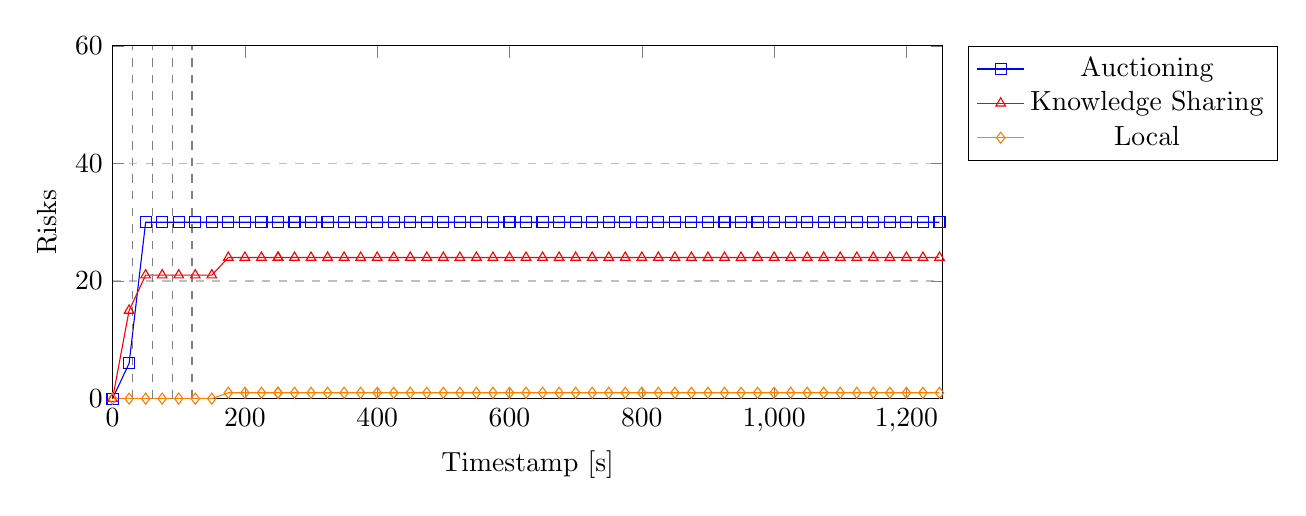
\begin{tikzpicture}
\begin{axis}[
    xlabel={Timestamp [s]},
    ylabel={Risks},
    xmin=0, xmax=1255000,
    ymin=0, ymax=60,
    legend pos=outer north east,
    ymajorgrids=true,
    grid style=dashed,
    width=\textwidth,
    height=0.5\textwidth,
    scaled x ticks=base 10:-3,
    xtick scale label code/.code={}
]

	\addplot[color=blue,mark=square] coordinates {
        (0,0)(25000,6)(50000,30)(75000,30)(100000,30)(125000,30)(150000,30)(175000,30)(200000,30)(225000,30)(250000,30)(275000,30)(300000,30)(325000,30)(350000,30)(375000,30)(400000,30)(425000,30)(450000,30)(475000,30)(500000,30)(525000,30)(550000,30)(575000,30)(600000,30)(625000,30)(650000,30)(675000,30)(700000,30)(725000,30)(750000,30)(775000,30)(800000,30)(825000,30)(850000,30)(875000,30)(900000,30)(925000,30)(950000,30)(975000,30)(1000000,30)(1025000,30)(1050000,30)(1075000,30)(1100000,30)(1125000,30)(1150000,30)(1175000,30)(1200000,30)(1225000,30)(1250000,30)(250362,30)
    };
    \addlegendentry{Auctioning}
	\addplot[color=red,mark=triangle] coordinates {
        (0,0)(25000,15)(50000,21)(75000,21)(100000,21)(125000,21)(150000,21)(175000,24)(200000,24)(225000,24)(250000,24)(275000,24)(300000,24)(325000,24)(350000,24)(375000,24)(400000,24)(425000,24)(450000,24)(475000,24)(500000,24)(525000,24)(550000,24)(575000,24)(600000,24)(625000,24)(650000,24)(675000,24)(700000,24)(725000,24)(750000,24)(775000,24)(800000,24)(825000,24)(850000,24)(875000,24)(900000,24)(925000,24)(950000,24)(975000,24)(1000000,24)(1025000,24)(1050000,24)(1075000,24)(1100000,24)(1125000,24)(1150000,24)(1175000,24)(1200000,24)(1225000,24)(1250000,24)(250334,24)
    };
    \addlegendentry{Knowledge Sharing}
	\addplot[color=orange,mark=diamond] coordinates {
        (0,0)(25000,0)(50000,0)(75000,0)(100000,0)(125000,0)(150000,0)(175000,1)(200000,1)(225000,1)(250000,1)(275000,1)(300000,1)(325000,1)(350000,1)(375000,1)(400000,1)(425000,1)(450000,1)(475000,1)(500000,1)(525000,1)(550000,1)(575000,1)(600000,1)(625000,1)(650000,1)(675000,1)(700000,1)(725000,1)(750000,1)(775000,1)(800000,1)(825000,1)(850000,1)(875000,1)(900000,1)(925000,1)(950000,1)(975000,1)(1000000,1)(1025000,1)(1050000,1)(1075000,1)(1100000,1)(1125000,1)(1150000,1)(1175000,1)(1200000,1)(1225000,1)(1250000,1)(250168,1)
    };
    \addlegendentry{Local}

	\addplot[color=gray, dashed,] coordinates {(30000,0) (30000,60)};
	\addplot[color=gray, dashed,] coordinates {(60000,0) (60000,60)};
	\addplot[color=gray, dashed,] coordinates {(90000,0) (90000,60)};
	\addplot[color=gray, dashed,] coordinates {(120000,0) (120000,60)};


\end{axis}
\end{tikzpicture}
    \caption{Graph showing the number of unique risks detected by agents in the unstable scenario.}
\end{figure}
\begin{figure}[H]
    \centering
        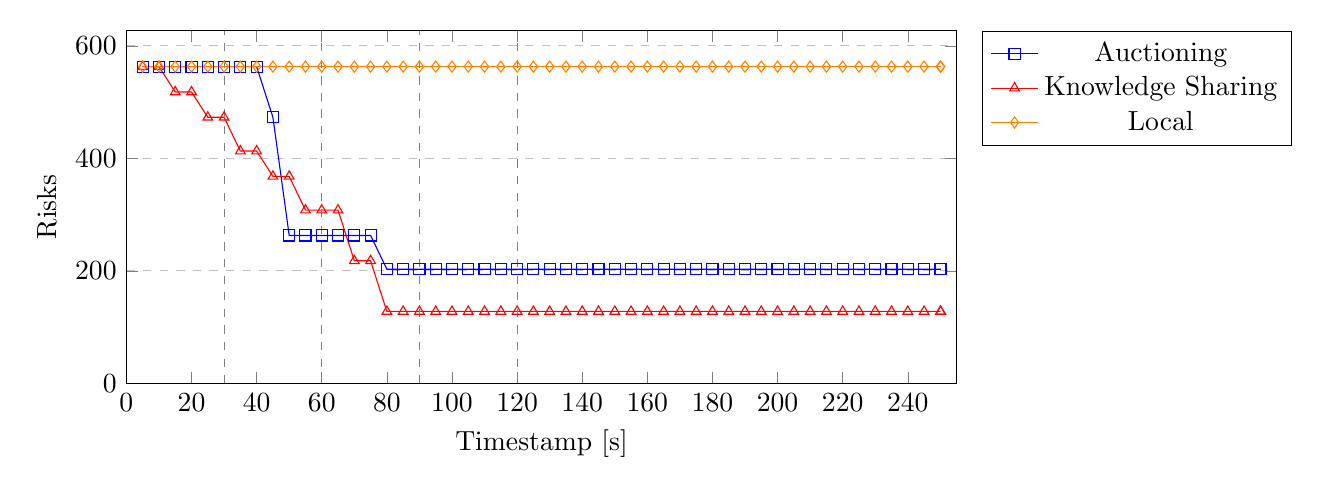
\begin{tikzpicture}
\begin{axis}[
    xlabel={Timestamp [s]},
    ylabel={Risks},
    xmin=0, xmax=255000,
    ymin=0, ymax=627,
    legend pos=outer north east,
    ymajorgrids=true,
    grid style=dashed,
    width=\textwidth,
    height=0.5\textwidth,
    scaled x ticks=base 10:-3,
    xtick scale label code/.code={}
]

	\addplot[color=blue,mark=square] coordinates {
        (5000,563)(10000,563)(15000,563)(20000,563)(25000,563)(30000,563)(35000,563)(40000,563)(45000,473)(50000,263)(55000,263)(60000,263)(65000,263)(70000,263)(75000,263)(80000,203)(85000,203)(90000,203)(95000,203)(100000,203)(105000,203)(110000,203)(115000,203)(120000,203)(125000,203)(130000,203)(135000,203)(140000,203)(145000,203)(150000,203)(155000,203)(160000,203)(165000,203)(170000,203)(175000,203)(180000,203)(185000,203)(190000,203)(195000,203)(200000,203)(205000,203)(210000,203)(215000,203)(220000,203)(225000,203)(230000,203)(235000,203)(240000,203)(245000,203)(250000,203)(250128,203)
    };
    \addlegendentry{Auctioning}
	\addplot[color=red,mark=triangle] coordinates {
        (5000,563)(10000,563)(15000,518)(20000,518)(25000,473)(30000,473)(35000,413)(40000,413)(45000,368)(50000,368)(55000,308)(60000,308)(65000,308)(70000,218)(75000,218)(80000,128)(85000,128)(90000,128)(95000,128)(100000,128)(105000,128)(110000,128)(115000,128)(120000,128)(125000,128)(130000,128)(135000,128)(140000,128)(145000,128)(150000,128)(155000,128)(160000,128)(165000,128)(170000,128)(175000,128)(180000,128)(185000,128)(190000,128)(195000,128)(200000,128)(205000,128)(210000,128)(215000,128)(220000,128)(225000,128)(230000,128)(235000,128)(240000,128)(245000,128)(250000,128)(250118,128)
    };
    \addlegendentry{Knowledge Sharing}
	\addplot[color=orange,mark=diamond] coordinates {
        (5000,563)(10000,563)(15000,563)(20000,563)(25000,563)(30000,563)(35000,563)(40000,563)(45000,563)(50000,563)(55000,563)(60000,563)(65000,563)(70000,563)(75000,563)(80000,563)(85000,563)(90000,563)(95000,563)(100000,563)(105000,563)(110000,563)(115000,563)(120000,563)(125000,563)(130000,563)(135000,563)(140000,563)(145000,563)(150000,563)(155000,563)(160000,563)(165000,563)(170000,563)(175000,563)(180000,563)(185000,563)(190000,563)(195000,563)(200000,563)(205000,563)(210000,563)(215000,563)(220000,563)(225000,563)(230000,563)(235000,563)(240000,563)(245000,563)(250000,563)(250107,563)
    };
    \addlegendentry{Local}

	\addplot[color=gray, dashed,] coordinates {(30000,0) (30000,627)};
	\addplot[color=gray, dashed,] coordinates {(60000,0) (60000,627)};
	\addplot[color=gray, dashed,] coordinates {(90000,0) (90000,627)};
	\addplot[color=gray, dashed,] coordinates {(120000,0) (120000,627)};


\end{axis}
\end{tikzpicture}
    \caption{Graph showing the number of remaining risks in the infrastructure in the unstable scenario.}
\end{figure}
\begin{figure}[H]
    \centering
        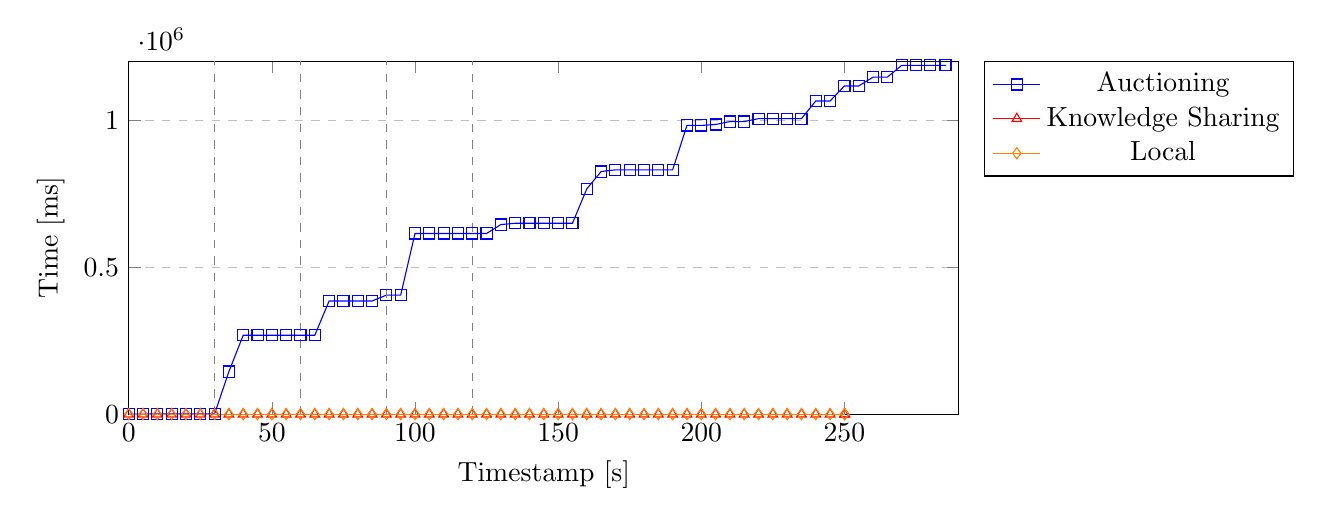
\begin{tikzpicture}
\begin{axis}[
    xlabel={Timestamp [s]},
    ylabel={Time [ms]},
    xmin=0, xmax=290000,
    ymin=0, ymax=1200012,
    legend pos=outer north east,
    ymajorgrids=true,
    grid style=dashed,
    width=\textwidth,
    height=0.5\textwidth,
    scaled x ticks=base 10:-3,
    xtick scale label code/.code={}
]

	\addplot[color=blue,mark=square] coordinates {
        (0,0)(5000,138)(10000,1198)(15000,1198)(20000,1198)(25000,1207)(30000,1207)(35000,144954)(40000,268597)(45000,268597)(50000,268597)(55000,268597)(60000,268597)(65000,268597)(70000,384913)(75000,384913)(80000,384919)(85000,384919)(90000,404941)(95000,404941)(100000,614605)(105000,614605)(110000,614608)(115000,614608)(120000,614609)(125000,614609)(130000,644926)(135000,649250)(140000,649250)(145000,649250)(150000,649251)(155000,649251)(160000,766138)(165000,825152)(170000,831011)(175000,831011)(180000,831012)(185000,831012)(190000,831012)(195000,982057)(200000,982057)(205000,985177)(210000,995185)(215000,995185)(220000,1005197)(225000,1005197)(230000,1005197)(235000,1005197)(240000,1065215)(245000,1065215)(250000,1116271)(255000,1116271)(260000,1146280)(265000,1146280)(270000,1186297)(275000,1186297)(280000,1186297)(285000,1186297)(285530,1186297)
    };
    \addlegendentry{Auctioning}
	\addplot[color=red,mark=triangle] coordinates {
        (0,0)(5000,0)(10000,0)(15000,0)(20000,0)(25000,0)(30000,0)(35000,0)(40000,0)(45000,0)(50000,0)(55000,0)(60000,0)(65000,0)(70000,0)(75000,0)(80000,0)(85000,0)(90000,0)(95000,0)(100000,0)(105000,0)(110000,0)(115000,0)(120000,0)(125000,0)(130000,0)(135000,0)(140000,0)(145000,0)(150000,0)(155000,0)(160000,0)(165000,0)(170000,0)(175000,0)(180000,0)(185000,0)(190000,0)(195000,0)(200000,0)(205000,0)(210000,0)(215000,0)(220000,0)(225000,0)(230000,0)(235000,0)(240000,0)(245000,0)(250000,0)(250138,0)
    };
    \addlegendentry{Knowledge Sharing}
	\addplot[color=orange,mark=diamond] coordinates {
        (0,0)(5000,0)(10000,0)(15000,0)(20000,0)(25000,0)(30000,0)(35000,0)(40000,0)(45000,0)(50000,0)(55000,0)(60000,0)(65000,0)(70000,0)(75000,0)(80000,0)(85000,0)(90000,0)(95000,0)(100000,0)(105000,0)(110000,0)(115000,0)(120000,0)(125000,0)(130000,0)(135000,0)(140000,0)(145000,0)(150000,0)(155000,0)(160000,0)(165000,0)(170000,0)(175000,0)(180000,0)(185000,0)(190000,0)(195000,0)(200000,0)(205000,0)(210000,0)(215000,0)(220000,0)(225000,0)(230000,0)(235000,0)(240000,0)(245000,0)(250000,0)(250134,0)
    };
    \addlegendentry{Local}

	\addplot[color=gray, dashed,] coordinates {(30000,0) (30000,1200012)};
	\addplot[color=gray, dashed,] coordinates {(60000,0) (60000,1200012)};
	\addplot[color=gray, dashed,] coordinates {(90000,0) (90000,1200012)};
	\addplot[color=gray, dashed,] coordinates {(120000,0) (120000,1200012)};


\end{axis}
\end{tikzpicture}
    \caption{Graph showing the sum of time spent auctioning by agents in the unstable scenario.}
\end{figure}
\begin{figure}[H]
    \centering
        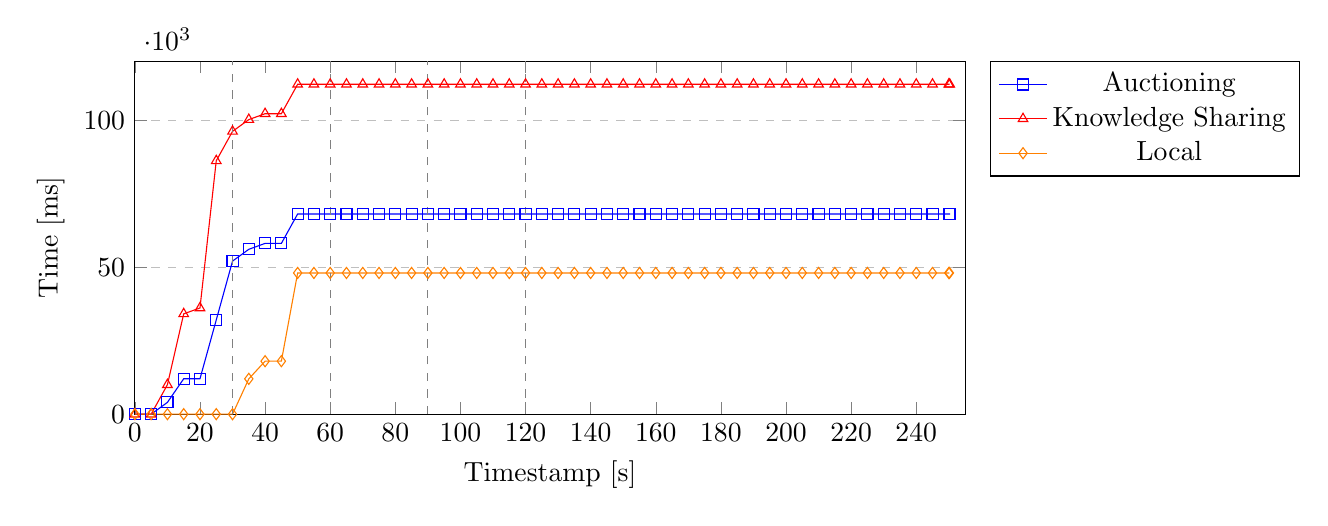
\begin{tikzpicture}
\begin{axis}[
    xlabel={Timestamp [s]},
    ylabel={Time [ms]},
    xmin=0, xmax=255000,
    ymin=0, ymax=120012,
    legend pos=outer north east,
    ymajorgrids=true,
    grid style=dashed,
    width=\textwidth,
    height=0.5\textwidth,
    scaled x ticks=base 10:-3,
    scaled y ticks=base 10:-3,
    xtick scale label code/.code={}
]

	\addplot[color=blue,mark=square] coordinates {
        (0,0)(5000,0)(10000,4012)(15000,12040)(20000,12040)(25000,32049)(30000,52060)(35000,56077)(40000,58088)(45000,58088)(50000,68099)(55000,68099)(60000,68099)(65000,68099)(70000,68099)(75000,68099)(80000,68099)(85000,68099)(90000,68099)(95000,68099)(100000,68099)(105000,68099)(110000,68099)(115000,68099)(120000,68099)(125000,68099)(130000,68099)(135000,68099)(140000,68099)(145000,68099)(150000,68099)(155000,68099)(160000,68099)(165000,68099)(170000,68099)(175000,68099)(180000,68099)(185000,68099)(190000,68099)(195000,68099)(200000,68099)(205000,68099)(210000,68099)(215000,68099)(220000,68099)(225000,68099)(230000,68099)(235000,68099)(240000,68099)(245000,68099)(250000,68099)(250367,68099)
    };
    \addlegendentry{Auctioning}
	\addplot[color=red,mark=triangle] coordinates {
        (0,0)(5000,0)(10000,10030)(15000,34121)(20000,36123)(25000,86181)(30000,96189)(35000,100197)(40000,102199)(45000,102199)(50000,112207)(55000,112207)(60000,112207)(65000,112207)(70000,112207)(75000,112207)(80000,112207)(85000,112207)(90000,112207)(95000,112207)(100000,112207)(105000,112207)(110000,112207)(115000,112207)(120000,112207)(125000,112207)(130000,112207)(135000,112207)(140000,112207)(145000,112207)(150000,112207)(155000,112207)(160000,112207)(165000,112207)(170000,112207)(175000,112207)(180000,112207)(185000,112207)(190000,112207)(195000,112207)(200000,112207)(205000,112207)(210000,112207)(215000,112207)(220000,112207)(225000,112207)(230000,112207)(235000,112207)(240000,112207)(245000,112207)(250000,112207)(250281,112207)
    };
    \addlegendentry{Knowledge Sharing}
	\addplot[color=orange,mark=diamond] coordinates {
        (0,0)(5000,0)(10000,0)(15000,0)(20000,0)(25000,0)(30000,0)(35000,12019)(40000,18027)(45000,18027)(50000,48034)(55000,48034)(60000,48034)(65000,48034)(70000,48034)(75000,48034)(80000,48034)(85000,48034)(90000,48034)(95000,48034)(100000,48034)(105000,48034)(110000,48034)(115000,48034)(120000,48034)(125000,48034)(130000,48034)(135000,48034)(140000,48034)(145000,48034)(150000,48034)(155000,48034)(160000,48034)(165000,48034)(170000,48034)(175000,48034)(180000,48034)(185000,48034)(190000,48034)(195000,48034)(200000,48034)(205000,48034)(210000,48034)(215000,48034)(220000,48034)(225000,48034)(230000,48034)(235000,48034)(240000,48034)(245000,48034)(250000,48034)(250187,48034)
    };
    \addlegendentry{Local}

	\addplot[color=gray, dashed,] coordinates {(30000,0) (30000,120012)};
	\addplot[color=gray, dashed,] coordinates {(60000,0) (60000,120012)};
	\addplot[color=gray, dashed,] coordinates {(90000,0) (90000,120012)};
	\addplot[color=gray, dashed,] coordinates {(120000,0) (120000,120012)};


\end{axis}
\end{tikzpicture}

    \caption{Graph showing the sum of time spent adapting by agents in the unstable scenario.}
\end{figure}
